



Electromagnetism is the theory of two vector fields -- the electric field and the magnetic field -- and of the charges which produce them and are pushed around by them. Between them, these fields are responsible for very nearly every phenomenon we encounter that is not gravity: the binding of electrons to nuclei and of atoms into molecules, the rigidity of solid objects, chemistry, electricity, magnets, and light itself.

What makes the subject beautiful, rather than merely useful, is that all of this is encoded in \emph{four} equations. Maxwell's equations are a system of linear partial differential equations relating the fields to their sources, and essentially the whole of this course consists of finding and interpreting their solutions. We will start with the static solutions -- stationary charges (electrostatics) and steady currents (magnetostatics) -- where the equations decouple and a great deal can be computed by hand. We will then let things depend on time, at which point the electric and magnetic fields become inextricably linked: changing magnetic fields drive currents, and the equations acquire wave solutions which travel at precisely the speed of light. Finally we will discover that the whole structure is really a relativistic one. Written in the language of special relativity, Maxwell's four equations collapse into two, and the magnetic field turns out to be nothing but the electric field seen by a moving observer.

This article constitutes my notes for the `Electromagnetism' course, held in Lent 2021 at Cambridge. These notes are \emph{not a transcription of the lectures}, and differ significantly in quite a few areas. Still, all lectured material should be covered. The reader is assumed to be comfortable with the vector calculus of the IA course -- gradients, divergences, curls, and the integral theorems of Green, Stokes and Gauss\footnote{The final section also uses special relativity at the level of the IA `Dynamics and Relativity' course, though we will review everything we need.}. If you spot any errors or have any feedback, I can be contacted at \href{mailto:ak2316@cam.ac.uk}{ak2316@cam.ac.uk}.



\section{Charges, Fields and Maxwell's Equations}

We begin by setting up the objects the theory is about. There are two kinds: the \emph{sources}, which are electric charges and their motion, and the \emph{fields}, which the sources produce and which in turn exert forces on the sources. The whole theory then amounts to two statements -- a force law telling us how fields push charges, and Maxwell's equations telling us how charges make fields.

\subsection{Charge and Charge Density}

Every particle carries a number, its \vocab{electric charge}, which measures how strongly it couples to the electromagnetic force. Charge is measured in Coulombs, and in this course we will happily allow it to be any real number. This is a lie, but a harmless one: at the fundamental level charge is quantised, and every particle carries $q = ne$ for some $n \in \Z$, where
$$
e \approx 1.6 \times 10^{-19}\,\mathrm{C}
$$
is the charge on a proton. The electron has $n = -1$, the proton $n = +1$, the neutron $n = 0$. Since $e$ is so tiny compared to the charges we deal with in practice, treating charge as a continuum is an excellent approximation, in exactly the same way that treating water as a continuous fluid is.

Rather than track individual particles, we therefore describe charge by a density.

\begin{definition}[Charge density]
	The \vocab{charge density} $\rho(\vv{x}, t)$ is the charge per unit volume, so that the total charge contained in a region $V \subseteq \R^3$ is
	$$
	Q = \int_V \rho(\vv{x}, t) \dd V.
	$$
\end{definition}

We will also want to consider idealised charge distributions which are concentrated on a surface, on a curve, or at a single point. In those cases the appropriate object is a charge per unit area $\sigma$, a charge per unit length $\eta$, or simply a charge $Q$ together with a delta function. Which one is meant will always be clear from context.

\subsection{Current and Current Density}

Charge that moves is a \emph{current}. Again the natural object is a density.

\begin{definition}[Current density]
	The \vocab{current density} $\vv{J}(\vv{x}, t)$ is a vector field with the property that, for any surface $S$,
	$$
	I = \int_S \vv{J} \cdot \dd \vv{S}
	$$
	is the charge crossing $S$ per unit time. The number $I$ is the \vocab{current} through $S$.
\end{definition}

So $\vv{J}$ points in the direction that charge is flowing, and its magnitude is the current per unit area. If the charge density $\rho$ is moving with velocity $\vv{v}(\vv{x}, t)$, then in time $\delta t$ the charge crossing a small patch of area $\delta A$ with unit normal $\hh{n}$ is the charge in a slanted cylinder of volume $(\vv{v} \cdot \hh{n})\delta A \, \delta t$, and so
$$
\vv{J} = \rho \vv{v}.
$$
This is worth remembering; it is the bridge between the field description and the particle description.

\begin{example}[Current in a wire]
	Consider a wire: a cylinder of cross-sectional area $A$ containing $n$ mobile electrons per unit volume, each of charge $q = -e$, all drifting along the wire with speed $v$. Then
	$$
	\rho = nq = -ne, \qquad \vv{J} = nq \vv{v}, \qquad I = |nqvA| = nevA.
	$$
	It is worth noting how slow this drift is in practice. For a copper wire of a square millimetre carrying an amp, $v$ works out at less than a tenth of a millimetre per second. The \emph{signal} travels essentially at the speed of light, but the electrons themselves shuffle along at a snail's pace.
\end{example}

\subsection{Conservation of Charge}

It is a fact of nature that charge cannot be created or destroyed. But this statement, as usually phrased, is much weaker than the truth. `The total charge in the universe is constant' would permit a charge to vanish from Cambridge and simultaneously appear on the Moon. What actually happens is that charge is conserved \emph{locally}: if the charge in some region decreases, it is because charge flowed out through the boundary.

The mathematical expression of this is a continuity equation, exactly as in the IA Vector Calculus course.

\begin{law}[Continuity equation]
	The charge density and current density satisfy
	$$
	\frac{\partial \rho}{\partial t} + \nabla \cdot \vv{J} = 0.
	$$
\end{law}

To see that this says what we claimed, fix a region $V$ with boundary $S = \partial V$ and let $Q(t) = \int_V \rho \dd V$ be the charge inside. Then differentiating under the integral sign and applying the divergence theorem,
$$
\frac{\dd Q}{\dd t} = \int_V \frac{\partial \rho}{\partial t} \dd V = -\int_V \nabla \cdot \vv{J} \dd V = - \int_S \vv{J} \cdot \dd \vv{S} = -I,
$$
where $I$ is the total current flowing out through $S$. In other words -- the charge in $V$ decreases at exactly the rate at which charge leaves through the boundary. Nothing teleports.

Taking $V = \R^3$ and assuming, as we always shall, that $\vv{J}$ decays at infinity, the surface term vanishes and we recover the global statement $\dd Q/\dd t = 0$. So local conservation implies global conservation, but not conversely.

\subsection{Fields and the Lorentz Force Law}

In modern physics we do not believe in action at a distance. Instead, forces are mediated by \emph{fields}: dynamical objects which assign a value to every point of space and time, and which carry energy and momentum in their own right. Electromagnetism has two of them,
$$
\vv{E}(\vv{x}, t) \quad \text{the \vocab{electric field}}, \qquad \vv{B}(\vv{x}, t) \quad \text{the \vocab{magnetic field}},
$$
both vector fields on $\R^3$.

The fields interact with charges in two directions, and it is worth keeping the two firmly separate in one's head.
\begin{itemize}
	\item Fields push charges. This is governed by the Lorentz force law.
	\item Charges make fields. This is governed by Maxwell's equations.
\end{itemize}

The first is quickly stated.

\begin{law}[Lorentz force law]
	A particle of charge $q$ moving with velocity $\vv{v}$ in fields $\vv{E}$ and $\vv{B}$ experiences a force
	$$
	\vv{F} = q\left(\vv{E} + \vv{v} \times \vv{B}\right).
	$$
\end{law}

Two features deserve immediate comment. The electric part $q\vv{E}$ acts on a charge whether or not it is moving, and points along $\vv{E}$. The magnetic part $q \vv{v} \times \vv{B}$ acts only on moving charges, and is perpendicular to the velocity. In particular
$$
\vv{F} \cdot \vv{v} = q(\vv{E} + \vv{v}\times \vv{B})\cdot \vv{v} = q \vv{E}\cdot \vv{v},
$$
so \emph{magnetic fields do no work}. They can bend a particle's trajectory but never change its speed. Every bit of energy a charged particle gains comes from the electric field.

For a continuous distribution of charge rather than a single particle, we should integrate. A volume element $\dd V$ carries charge $\rho \dd V$ moving with velocity $\vv{v}$, so it feels a force $(\rho \vv{E} + \rho \vv{v}\times \vv{B})\dd V$, giving
$$
\vv{F} = \int_V \left(\rho \vv{E} + \vv{J} \times \vv{B}\right) \dd V
$$
using $\vv{J} = \rho \vv{v}$. We will use the magnetic half of this repeatedly when we compute forces between wires.

\subsection{Maxwell's Equations}

Now for the other half of the story: how charges produce fields. Remarkably, the answer fits on one line each.

\begin{law}[Maxwell's equations]
	\label{law:maxwell}
	The electromagnetic fields produced by a charge density $\rho$ and current density $\vv{J}$ obey
	\begin{align*}
		\nabla \cdot \vv{E} &= \frac{\rho}{\epsilon_0}, \tag{M1}\\
		\nabla \cdot \vv{B} &= 0, \tag{M2}\\
		\nabla \times \vv{E} + \frac{\partial \vv{B}}{\partial t} &= \vv{0}, \tag{M3}\\
		\nabla \times \vv{B} - \mu_0 \epsilon_0 \frac{\partial \vv{E}}{\partial t} &= \mu_0 \vv{J}. \tag{M4}
	\end{align*}
	Here $\epsilon_0$ and $\mu_0$ are constants of nature, the \vocab{electric constant} and the \vocab{magnetic constant}\footnote{These are also called the permittivity and permeability of free space, which sound more impressive but mean the same thing.}, with numerical values
	$$
	\epsilon_0 \approx 8.85 \times 10^{-12}\,\mathrm{m}^{-3}\,\mathrm{kg}^{-1}\,\mathrm{s}^{2}\,\mathrm{C}^{2}, \qquad \mu_0 = 4\pi \times 10^{-7}\,\mathrm{m}\,\mathrm{kg}\,\mathrm{C}^{-2}.
	$$
\end{law}

That is the entire content of classical electromagnetism. Everything that follows in this course -- Coulomb's law, capacitors, solenoids, induction, light -- is a consequence of these four equations together with the Lorentz force law. It is genuinely astonishing that so much should follow from so little, and the reader is encouraged to keep the equations somewhere visible while reading the rest of these notes.

A few structural remarks before we start solving them.

\emph{They are linear.} If $(\vv{E}_1, \vv{B}_1)$ solves the equations with sources $(\rho_1, \vv{J}_1)$ and $(\vv{E}_2, \vv{B}_2)$ solves them with sources $(\rho_2, \vv{J}_2)$, then the sum solves them with the summed sources. This is the \vocab{principle of superposition}, and it is why electromagnetism is tractable at all. Of the four fundamental forces, it is the only one with this property.

\emph{They are inconsistent without the last term.} Take the divergence of (M4). Since $\nabla \cdot (\nabla \times \vv{B}) = 0$ always,
$$
0 = \mu_0 \epsilon_0 \frac{\partial}{\partial t}(\nabla \cdot \vv{E}) + \mu_0 \nabla \cdot \vv{J} = \mu_0\left(\frac{\partial \rho}{\partial t} + \nabla \cdot \vv{J}\right),
$$
where we used (M1) in the last step. So Maxwell's equations do not merely permit charge conservation -- they \emph{imply} it. We will see in Section~\ref{sec:displacement} that had we written (M4) without the $\partial \vv{E}/\partial t$ term (which is what Amp\`ere originally wrote), the same computation would have forced $\partial \rho/\partial t = 0$, which is plainly false. The extra term is Maxwell's, and it is also, as we shall see, the term responsible for light.

\emph{They come in pairs.} Equations (M2) and (M3) contain no sources at all: they are constraints on the fields themselves, and they are exactly the conditions which allow us to introduce potentials. Equations (M1) and (M4) are the ones that say where the fields come from.

\emph{They have an integral form.} Applying the integral theorems to each gives a statement with a direct physical reading; we will derive each in turn as we meet it, but for reference the four integral forms are
\begin{align*}
	\int_{\partial V} \vv{E}\cdot \dd \vv{S} &= \frac{Q}{\epsilon_0}, & &\text{(Gauss' law)}\\
	\int_{\partial V} \vv{B}\cdot \dd \vv{S} &= 0, & &\text{(no magnetic monopoles)}\\
	\oint_{\partial S} \vv{E} \cdot \dd \vv{x} &= -\frac{\dd}{\dd t}\int_S \vv{B}\cdot \dd \vv{S}, & &\text{(Faraday's law)}\\
	\oint_{\partial S} \vv{B} \cdot \dd \vv{x} &= \mu_0 \int_S \vv{J}\cdot \dd \vv{S} + \mu_0\epsilon_0 \frac{\dd}{\dd t}\int_S \vv{E}\cdot \dd \vv{S}. & &\text{(Amp\`ere's law)}
\end{align*}
The reader who has done the IA Vector Calculus course will have seen a version of this already; we now do the whole thing properly.

\subsection{The Static Limit}

The most important simplification is to look for solutions which do not depend on time. Setting all time derivatives to zero, Maxwell's equations fall apart into two entirely independent systems:
$$
\begin{cases}
	\nabla \cdot \vv{E} = \rho/\epsilon_0, \\
	\nabla \times \vv{E} = \vv{0},
\end{cases}
\qquad \qquad
\begin{cases}
	\nabla \cdot \vv{B} = 0, \\
	\nabla \times \vv{B} = \mu_0 \vv{J}.
\end{cases}
$$
The first pair involves only $\vv{E}$ and $\rho$; the second only $\vv{B}$ and $\vv{J}$. This is the sense in which electricity and magnetism are separate phenomena in the static world -- they only become entangled once things start changing in time. Accordingly we spend the next two sections on \vocab{electrostatics} (stationary charges, $\rho = \rho(\vv{x})$, $\vv{J} = \vv{0}$) and \vocab{magnetostatics} (steady currents, $\rho = 0$, $\vv{J} = \vv{J}(\vv{x})$) respectively, and only afterwards let time back in.

\section{Electrostatics}

In electrostatics nothing moves. We take $\vv{J} = \vv{0}$, we take $\rho = \rho(\vv{x})$ independent of time, and we look for a time-independent electric field with $\vv{B} = \vv{0}$. As we saw, the equations we have to solve are
$$
\nabla \cdot \vv{E} = \frac{\rho}{\epsilon_0}, \qquad \nabla \times \vv{E} = \vv{0},
$$
and (M2) and (M4) are satisfied trivially. The goal of this section is to determine $\vv{E}$ from $\rho$: first in highly symmetric situations, where a single application of the divergence theorem does everything, and then in general.

\subsection{Gauss' Law}

The integral form of (M1) is so useful that it gets its own name. Let $V$ be a region with boundary $S = \partial V$. Integrating (M1) over $V$,
$$
\int_V \nabla \cdot \vv{E} \dd V = \frac{1}{\epsilon_0}\int_V \rho \dd V,
$$
and applying the divergence theorem on the left gives the following.

\begin{law}[Gauss' law]
	For any closed surface $S$ bounding a region $V$,
	$$
	\int_S \vv{E} \cdot \dd \vv{S} = \frac{Q}{\epsilon_0},
	$$
	where $Q = \int_V \rho \dd V$ is the total charge enclosed by $S$.
\end{law}

\begin{definition}[Flux]
	The \vocab{flux} of $\vv{E}$ through a surface $S$ is $\int_S \vv{E}\cdot \dd \vv{S}$.
\end{definition}

Gauss' law says something slightly surprising. The flux out of $S$ depends only on the charge \emph{inside} $S$, and not at all on the charge outside. This is not to say that external charges make no field on $S$ -- of course they do -- but their field lines enter through one part of the surface and leave through another, and the two contributions cancel exactly.

The reason Gauss' law is so powerful is that, when the charge distribution has enough symmetry, symmetry alone determines the direction of $\vv{E}$ and the surfaces on which $|\vv{E}|$ is constant. Gauss' law then determines the one remaining unknown function. Let's see this in action.

\begin{example}[Coulomb's law]
	Take a spherically symmetric charge distribution $\rho = \rho(r)$ with $\rho(r) = 0$ for $r > R$, so all the charge lies inside a ball of radius $R$, and let $Q$ be the total charge. We take for $S$ a sphere of radius $r > R$ centred at the origin.

	\begin{center}
	\begin{tikzpicture}[scale=1.0]
		\fill[gray!15] (0,0) circle (1);
		\draw (0,0) circle (1);
		\draw[->] (0,0) -- (0.707,0.707) node[midway, anchor=south east, inner sep=1pt] {$R$};
		\draw[dashed, figred] (0,0) circle (1.6);
		\node[figred, anchor=south east, inner sep=1pt] at (-1.13,1.13) {$S$};
		\foreach \a in {0,45,...,315}
			\draw[->, blue] (\a:1.7) -- (\a:2.35);
		\node[blue, anchor=west, inner sep=2pt] at (2.35,0) {$\vv{E}$};
		\draw[->] (0,0) -- (200:1.6) node[midway, anchor=south west, inner sep=1pt] {$r$};
	\end{tikzpicture}
	\end{center}

	By symmetry the field can only point radially and can only depend on $r$, so
	$$
	\vv{E} = E(r)\hh{r}.
	$$
	(Note this automatically has $\nabla \times \vv{E} = \vv{0}$, so we need only worry about (M1).) The flux is then
	$$
	\int_S \vv{E}\cdot \dd \vv{S} = \int_S E(r)\, \hh{r}\cdot \dd \vv{S} = E(r) \cdot 4\pi r^2,
	$$
	since $\hh{r}$ is precisely the outward normal to $S$ and $E(r)$ is constant on $S$. Gauss' law now gives $4\pi r^2 E(r) = Q/\epsilon_0$, so
	$$
	\vv{E}(\vv{r}) = \frac{Q}{4\pi \epsilon_0 r^2}\hh{r}, \qquad r > R.
	$$
	Combining with the Lorentz force law, a second charge $q$ placed at $\vv{r}$ feels a force
	$$
	\vv{F} = \frac{Qq}{4\pi\epsilon_0 r^2}\hh{r},
	$$
	which is \vocab{Coulomb's law}: an inverse square law, repulsive for like charges and attractive for unlike ones. It is worth pausing over the fact that we never needed to know $\rho(r)$, only the total charge $Q$. From outside, any spherically symmetric lump of charge is indistinguishable from a point charge at its centre.
\end{example}

\begin{example}[Inside a uniformly charged ball]
	Now take the charge to be uniformly spread through the ball,
	$$
	\rho(r) = \begin{cases} \rho_0 & r < R,\\ 0 & r > R,\end{cases}
	$$
	with total charge $Q = \frac{4}{3}\pi R^3 \rho_0$, and ask what happens \emph{inside}. Take $S$ to be a sphere of radius $r < R$.

	\begin{center}
	\begin{tikzpicture}[scale=1.0]
		\fill[gray!15] (0,0) circle (1.6);
		\draw (0,0) circle (1.6);
		\draw[->] (0,0) -- (60:1.6) node[midway, anchor=south east, inner sep=1pt] {$R$};
		\draw[dashed, figred] (0,0) circle (0.85);
		\node[figred, anchor=north west, inner sep=1pt] at (0.60,-0.60) {$S$};
		\draw[->] (0,0) -- (160:0.85) node[midway, anchor=south, inner sep=1pt] {$r$};
		\foreach \a in {0,45,...,315}
			\draw[->, blue] (\a:1.75) -- (\a:2.4);
		\node[blue, anchor=west, inner sep=2pt] at (2.4,0) {$\vv{E}$};
	\end{tikzpicture}
	\end{center}

	The charge enclosed is now only $Q r^3/R^3$, so Gauss' law reads
	$$
	4\pi r^2 E(r) = \frac{Q}{\epsilon_0}\frac{r^3}{R^3},
	$$
	giving
	$$
	\vv{E}(\vv{r}) = \frac{Qr}{4\pi \epsilon_0 R^3}\hh{r}, \qquad r < R.
	$$
	So inside the ball the field grows \emph{linearly} with $r$, reaching its maximum on the surface $r = R$, where it matches continuously onto the exterior solution $Q/4\pi\epsilon_0 r^2$ found above. It vanishes at the centre, as it must by symmetry.
\end{example}

\begin{example}[Line charge]
	Consider an infinite straight line of charge along the $z$-axis, with uniform charge per unit length $\eta$. We use cylindrical polars $(r, \varphi, z)$.

	\begin{center}
	\begin{tikzpicture}[scale=1.0]
		\draw[thick] (0,-2.2) -- (0,2.2) node[above, inner sep=2pt] {$z$};
		% cylinder
		\draw[figred, dashed] (0.75,1.4) arc (0:180:0.75 and 0.24);
		\draw[figred] (-0.75,1.4) arc (180:360:0.75 and 0.24);
		\draw[figred] (-0.75,1.4) -- (-0.75,-1.4);
		\draw[figred] (0.75,1.4) -- (0.75,-1.4);
		\draw[figred, dashed] (0.75,-1.4) arc (0:180:0.75 and 0.24);
		\draw[figred] (-0.75,-1.4) arc (180:360:0.75 and 0.24);
		\node[figred, anchor=north east, inner sep=4pt] at (-0.55,-1.55) {$S$};
		\foreach \z in {-0.8,0,0.8} {
			\draw[->, blue] (0.82,\z) -- (2.1,\z);
			\draw[->, blue] (-0.82,\z) -- (-2.1,\z);
		}
		\node[blue, anchor=south, inner sep=2pt] at (1.7,0.85) {$\vv{E}$};
		\draw[<->] (2.5,-1.4) -- (2.5,1.4) node[midway, anchor=west, inner sep=2pt] {$L$};
	\end{tikzpicture}
	\end{center}

	By symmetry (translations along $z$, rotations about $z$, and reflection in any plane containing the axis) the field must be radial and depend only on $r$:
	$$
	\vv{E} = E(r)\hh{r}.
	$$
	Take $S$ to be a cylinder of radius $r$ and length $L$ about the axis. The end caps contribute nothing, since $\vv{E}$ is tangent to them, and the curved part has area $2\pi r L$ with outward normal $\hh{r}$. So
	$$
	\int_S \vv{E}\cdot \dd \vv{S} = 2\pi r L\, E(r) = \frac{\eta L}{\epsilon_0},
	$$
	giving
	$$
	\vv{E} = \frac{\eta}{2\pi \epsilon_0 r}\hh{r}.
	$$
	Note that the field falls off like $1/r$ rather than $1/r^2$. This is exactly what one should expect: we have one extra dimension's worth of charge contributing, so the field dies away more slowly.
\end{example}

\begin{example}[Plane of charge]
	Finally, let all the charge sit on the plane $z = 0$ with uniform charge per unit area $\sigma$.

	\begin{center}
	\begin{tikzpicture}[scale=1.0]
		\fill[gray!15] (-2.9,-0.55) -- (1.1,-0.55) -- (2.9,0.55) -- (-1.1,0.55) -- cycle;
		\draw (-2.9,-0.55) -- (1.1,-0.55) -- (2.9,0.55) -- (-1.1,0.55) -- cycle;
		\foreach \x in {-1.8,-1.05,1.5} {
			\draw[->, blue] (\x,0.3) -- (\x,1.5);
			\draw[->, blue] (\x,-0.3) -- (\x,-1.5);
		}
		\node[blue, anchor=west, inner sep=3pt] at (1.52,1.3) {$\vv{E}$};
		% pillbox
		\draw[figred] (-0.6,1.25) arc (180:360:0.6 and 0.19);
		\draw[figred, dashed] (-0.6,1.25) arc (180:0:0.6 and 0.19);
		\draw[figred] (-0.6,1.25) -- (-0.6,-1.25);
		\draw[figred] (0.6,1.25) -- (0.6,-1.25);
		\draw[figred] (-0.6,-1.25) arc (180:360:0.6 and 0.19);
		\draw[figred, dashed] (-0.6,-1.25) arc (180:0:0.6 and 0.19);
		\node[figred, anchor=north, inner sep=4pt] at (0,-1.5) {$S$};
		\draw[<->] (-0.6,0) -- (0.6,0) node[midway, anchor=south, inner sep=1pt] {\small $A$};
	\end{tikzpicture}
	\end{center}

	By symmetry the field is vertical and depends only on $z$, and reflection in the plane forces it to be odd:
	$$
	\vv{E} = E(z)\hh{z}, \qquad E(-z) = -E(z).
	$$
	Take for $S$ a cylinder (a `Gaussian pillbox') of cross-sectional area $A$ with its flat faces at heights $\pm z$. Now it is the curved side that contributes nothing, and the two caps that do:
	$$
	\int_S \vv{E}\cdot \dd \vv{S} = E(z)A - E(-z)A = 2E(z)A = \frac{\sigma A}{\epsilon_0}.
	$$
	Hence
	$$
	E(z) = \frac{\sigma}{2\epsilon_0} \quad \text{for } z > 0,
	$$
	which is \emph{constant} -- the field of an infinite charged plane does not decay at all. (Each successive dimension of charge costs us one power of $r$, and we have run out of powers.)
\end{example}

The last example exhibits an important general phenomenon: $\vv{E}$ jumps across a layer of surface charge. Here
$$
E(0^+) - E(0^-) = \frac{\sigma}{\epsilon_0},
$$
and this is not special to the plane.

\begin{proposition}[Discontinuity across a surface charge]
	\label{prop:jump-E}
	Let $S$ be a surface carrying surface charge density $\sigma$, with unit normal $\hh{n}$ pointing from the $-$ side to the $+$ side. Then
	$$
	\hh{n}\cdot \vv{E}_+ - \hh{n}\cdot\vv{E}_- = \frac{\sigma}{\epsilon_0},
	$$
	while the components of $\vv{E}$ tangential to $S$ are continuous.
\end{proposition}
\begin{proof}
	For the normal component, apply Gauss' law to a small pillbox straddling $S$, with flat faces of area $\delta A$ parallel to $S$ on either side, and then shrink the height of the pillbox to zero. The contribution of the curved side vanishes in the limit, the enclosed charge tends to $\sigma \, \delta A$, and the two faces contribute $(\hh{n}\cdot \vv{E}_+ - \hh{n}\cdot \vv{E}_-)\delta A$. Dividing by $\delta A$ gives the result.

	For the tangential component, use $\nabla \times \vv{E} = \vv{0}$ instead. Take a small rectangular loop $C$ straddling $S$, with two sides of length $\delta \ell$ parallel to $S$ (one either side) and two short sides crossing it, and let $\hh{t}$ be the unit tangent along the long sides. By Stokes' theorem $\oint_C \vv{E}\cdot \dd \vv{x} = \int (\nabla \times \vv{E})\cdot \dd \vv{S} = 0$. Shrinking the short sides to zero length leaves $(\hh{t}\cdot \vv{E}_+ - \hh{t}\cdot \vv{E}_-)\delta \ell = 0$, and since $\hh{t}$ was an arbitrary tangent direction, the tangential components agree.
\end{proof}

\subsection{The Electrostatic Potential}

Symmetry will only take us so far. To handle a general $\rho$ we must actually solve
$$
\nabla \cdot \vv{E} = \frac{\rho}{\epsilon_0}, \qquad \nabla \times \vv{E} = \vv{0}.
$$
The trick, familiar from vector calculus, is that the second equation solves itself. A curl-free field on $\R^3$ (which is simply connected) is a gradient.

\begin{definition}[Electrostatic potential]
	If $\vv{E} = -\nabla \phi$, we call the scalar field $\phi$ the \vocab{electrostatic potential}.
\end{definition}

The minus sign is a convention, and a sensible one: it makes $\phi$ agree with potential energy per unit charge, so that positive charges roll downhill. Substituting into (M1) turns the whole of electrostatics into a single scalar equation.

\begin{proposition}[Poisson's equation]
	The electrostatic potential satisfies
	$$
	\nabla^2 \phi = -\frac{\rho}{\epsilon_0}.
	$$
	In a region free of charge this reduces to \vocab{Laplace's equation} $\nabla^2 \phi = 0$.
\end{proposition}

Two remarks. First, $\phi$ is only determined up to an additive constant, since $\nabla$ kills constants. We fix this in the usual way by demanding $\phi(\vv{r}) \to 0$ as $r \to \infty$, which is possible whenever the charge is confined to a bounded region. Secondly, Poisson's equation is linear, which is superposition again: the potential of a collection of charges is the sum of the individual potentials.

Poisson's equation was studied at length in the IA Vector Calculus course, and we will lean on it heavily. The single most useful fact is the uniqueness theorem, which is worth recalling in full since we will use it to justify some outrageous-looking guesses later on.

\begin{theorem}[Uniqueness for Poisson's equation]
	\label{thm:uniqueness}
	Let $V$ be a bounded region with boundary $\partial V$, and consider the problem
	$$
	\nabla^2 \phi = -\frac{\rho}{\epsilon_0} \quad \text{in } V,
	$$
	subject to either $\phi$ specified on $\partial V$ (Dirichlet conditions) or $\partial \phi/\partial n = \hh{n}\cdot\nabla\phi$ specified on $\partial V$ (Neumann conditions). Then the solution is unique -- in the Dirichlet case outright, and in the Neumann case up to an additive constant.
\end{theorem}
\begin{proof}
	Suppose $\phi_1$ and $\phi_2$ are both solutions, and set $\psi = \phi_1 - \phi_2$. Then $\nabla^2 \psi = 0$ in $V$, and on $\partial V$ we have either $\psi = 0$ (Dirichlet) or $\partial \psi/\partial n = 0$ (Neumann). Now consider
	$$
	\int_V \nabla\cdot(\psi \nabla \psi)\dd V = \int_V \left(|\nabla \psi|^2 + \psi \nabla^2 \psi\right)\dd V = \int_V |\nabla\psi|^2 \dd V,
	$$
	using harmonicity of $\psi$. On the other hand, by the divergence theorem the left hand side is
	$$
	\int_{\partial V} \psi \nabla \psi \cdot \dd \vv{S} = \int_{\partial V}\psi \frac{\partial \psi}{\partial n}\dd S = 0,
	$$
	since one factor or the other vanishes on $\partial V$ in each case. Hence $\int_V |\nabla\psi|^2 \dd V = 0$, and as the integrand is non-negative and continuous, $\nabla \psi = \vv{0}$ throughout $V$. So $\psi$ is constant, and in the Dirichlet case that constant is zero.
\end{proof}

The theorem also holds on unbounded regions provided we impose a decay condition at infinity, which for us will always be $\phi \to 0$ as $r \to \infty$. The moral is a practical one: if by any means whatsoever -- inspired guesswork included -- we produce a function satisfying the equation and the boundary conditions, we have found \emph{the} answer, and are not obliged to explain how we found it.

\begin{example}[The point charge, again]
	A point charge $Q$ at the origin has
	$$
	\rho(\vv{r}) = Q\, \delta^3(\vv{r}),
	$$
	where $\delta^3$ is the three-dimensional delta function. Away from the origin we must solve Laplace's equation with spherical symmetry, and the general such solution is $\phi = \alpha/r + \text{const}$; the constant is zero by our boundary condition at infinity.

	To fix $\alpha$, integrate Poisson's equation over a ball $V$ of radius $r$. The left hand side is
	$$
	\int_V \nabla^2 \phi \dd V = \int_S \nabla \phi \cdot \dd \vv{S} = \int_S \left(-\frac{\alpha}{r^2}\right)\hh{r}\cdot \dd \vv{S} = -4\pi \alpha,
	$$
	while the right hand side is $-Q/\epsilon_0$. Hence $\alpha = Q/4\pi\epsilon_0$, and
	$$
	\phi = \frac{Q}{4\pi\epsilon_0 r}, \qquad \vv{E} = -\nabla \phi = \frac{Q}{4\pi \epsilon_0 r^2}\hh{r},
	$$
	which is Coulomb's law once more, now derived by a completely different route.
\end{example}

\subsection{General Charge Distributions}

The point charge solution is the key to everything else, because it is (up to a constant) the Green's function for the Laplacian. Recall that this is the function $G$ solving
$$
\nabla^2 G(\vv{r}; \vv{r}') = \delta^3(\vv{r}-\vv{r}'),
$$
and the calculation we just did says
$$
G(\vv{r}; \vv{r}') = -\frac{1}{4\pi}\frac{1}{|\vv{r}-\vv{r}'|}.
$$

\begin{proposition}[Potential of a general distribution]
	\label{prop:general-phi}
	Let $\rho$ be a charge distribution confined to a bounded region $V$. Then
	$$
	\phi(\vv{r}) = \frac{1}{4\pi\epsilon_0}\int_V \frac{\rho(\vv{r}')}{|\vv{r}-\vv{r}'|}\dd V',
	$$
	and correspondingly
	$$
	\vv{E}(\vv{r}) = \frac{1}{4\pi \epsilon_0}\int_V \rho(\vv{r}')\frac{\vv{r}-\vv{r}'}{|\vv{r}-\vv{r}'|^3}\dd V'.
	$$
\end{proposition}
\begin{proof}
	Since $\nabla^2 \phi = -\rho/\epsilon_0$ and $G$ is the Green's function,
	$$
	\phi(\vv{r}) = -\frac{1}{\epsilon_0}\int_V \rho(\vv{r}') G(\vv{r};\vv{r}')\dd V' = \frac{1}{4\pi \epsilon_0}\int_V \frac{\rho(\vv{r}')}{|\vv{r}-\vv{r}'|}\dd V'.
	$$
	For the field we differentiate under the integral sign, noting that $\nabla$ acts on $\vv{r}$ only, and
	$$
	\nabla\left(\frac{1}{|\vv{r}-\vv{r}'|}\right) = -\frac{\vv{r}-\vv{r}'}{|\vv{r}-\vv{r}'|^3}.
	$$
	Then $\vv{E} = -\nabla \phi$ gives the stated formula.
\end{proof}

This is a complete answer, but for a complicated $\rho$ it is a complete answer of the least useful kind: an integral one cannot do. What saves us is that we are usually far away from the charge, and then we can expand.

\subsection{The Multipole Expansion and Dipoles}

Suppose all the charge lies within some bounded region near the origin, and we look at the potential at $|\vv{r}| \gg |\vv{r}'|$. Taylor expanding the Green's function in $\vv{r}'$,
$$
\frac{1}{|\vv{r}-\vv{r}'|} = \frac{1}{r} + \frac{\vv{r}\cdot \vv{r}'}{r^3} + O\!\left(\frac{r'^2}{r^3}\right),
$$
and substituting into Proposition~\ref{prop:general-phi} gives
$$
\phi(\vv{r}) = \frac{1}{4\pi \epsilon_0}\left(\frac{Q}{r} + \frac{\vv{p}\cdot \hh{r}}{r^2} + \cdots\right),
$$
where
$$
Q = \int_V \rho(\vv{r}')\dd V', \qquad \vv{p} = \int_V \vv{r}'\, \rho(\vv{r}')\dd V'.
$$
This is the beginning of the \vocab{multipole expansion}. The leading term says that from far enough away any lump of charge looks like a point charge with the same total charge. The correction $\vv{p}$ is the first thing you see when the total charge vanishes.

\begin{definition}[Electric dipole moment]
	The \vocab{electric dipole moment} of a charge distribution is
	$$
	\vv{p} = \int \vv{r}'\rho(\vv{r}')\dd V'.
	$$
\end{definition}

Note that $\vv{p}$ depends on the choice of origin in general -- but if $Q = 0$, shifting the origin by $\vv{a}$ changes $\vv{p}$ by $-\vv{a}Q = \vv{0}$, so for a neutral distribution the dipole moment is well defined. This is the case of interest.

The cleanest example is a pair of equal and opposite point charges.

\begin{example}[The dipole]
	Put a charge $+Q$ at the origin and $-Q$ at $-\vv{d}$. By superposition,
	$$
	\phi(\vv{r}) = \frac{Q}{4\pi\epsilon_0}\left(\frac{1}{r} - \frac{1}{|\vv{r}+\vv{d}|}\right).
	$$
	This is exact but unenlightening; we expand for $r \gg d$. Using the general Taylor expansion $f(\vv{r}+\vv{d}) = f(\vv{r}) + \vv{d}\cdot \nabla f + \tfrac{1}{2}(\vv{d}\cdot \nabla)^2 f + \cdots$ with $f = 1/r$,
	$$
	\frac{1}{|\vv{r}+\vv{d}|} = \frac{1}{r} - \frac{\vv{d}\cdot \vv{r}}{r^3} + O\!\left(\frac{d^2}{r^3}\right),
	$$
	so the $1/r$ terms cancel and
	$$
	\phi(\vv{r}) \approx \frac{Q}{4\pi\epsilon_0}\frac{\vv{d}\cdot \vv{r}}{r^3} = \frac{\vv{p}\cdot \hh{r}}{4\pi\epsilon_0 r^2}, \qquad \vv{p} = Q\vv{d}.
	$$
	This agrees with our general formula, as it must. Note the convention: $\vv{p}$ points from the negative charge to the positive one.

	Differentiating, and using $\nabla(\vv{p}\cdot \vv{r}) = \vv{p}$ and $\nabla(r^{-3}) = -3\hh{r}/r^4$,
	$$
	\vv{E} = -\nabla \phi = \frac{1}{4\pi \epsilon_0}\left(\frac{3(\vv{p}\cdot \hh{r})\hh{r} - \vv{p}}{r^3}\right).
	$$
	So the dipole field falls off like $1/r^3$, faster than a point charge, which is unsurprising: at large distances the two charges nearly cancel.
\end{example}

Dipoles are not only things that produce fields; they are also things that respond to them, and the way they do so explains a good deal of everyday physics.

\begin{proposition}[Dipole in an external field]
	\label{prop:dipole-external}
	A dipole $\vv{p}$ sitting in an external field $\vv{E}$ has potential energy
	$$
	U = -\vv{p}\cdot\vv{E},
	$$
	experiences a torque
	$$
	\vv{\tau} = \vv{p}\times \vv{E}
	$$
	about its centre, and (if the field is non-uniform) a net force
	$$
	\vv{F} = \nabla(\vv{p}\cdot\vv{E}).
	$$
\end{proposition}
\begin{proof}
	Model the dipole as charges $\pm Q$ at $\vv{r}\pm\tfrac12\vv{d}$, with $\vv{p} = Q\vv{d}$. The total energy in the external potential $\phi$ is
	$$
	U = Q\phi(\vv{r}+\tfrac12\vv{d}) - Q\phi(\vv{r}-\tfrac12\vv{d}) = Q\,\vv{d}\cdot\nabla\phi(\vv{r}) + O(d^2) = -\vv{p}\cdot\vv{E}(\vv{r}),
	$$
	Taylor expanding and using $\vv{E} = -\nabla\phi$. The force is minus the gradient of the energy, $\vv{F} = -\nabla U = \nabla(\vv{p}\cdot\vv{E})$, which indeed vanishes for a uniform field. For the torque, the two charges feel forces $\pm Q\vv{E}$, so about the centre
	$$
	\vv{\tau} = \tfrac12\vv{d}\times(Q\vv{E}) + (-\tfrac12\vv{d})\times(-Q\vv{E}) = Q\vv{d}\times\vv{E} = \vv{p}\times\vv{E}. \qedhere
	$$
\end{proof}

The energy $-\vv{p}\cdot\vv{E}$ is minimised when $\vv{p}$ is aligned with $\vv{E}$, and the torque is exactly what rotates it into alignment. This is the mechanism behind a great deal of chemistry -- a water molecule is a permanent dipole, and it is why microwave ovens work and why water is such a good solvent. The force formula also explains why a charged comb picks up small neutral pieces of paper: the field of the comb \emph{induces} a dipole in the paper, and being non-uniform, then pulls on it.

\subsection{Field Lines and Equipotentials}

Drawing a vector field is awkward -- we cannot draw an arrow at every point. The standard device is to draw \emph{field lines} instead.

\begin{definition}[Field lines and equipotentials]
	A \vocab{field line} is a curve everywhere tangent to $\vv{E}$, drawn with the convention that the density of lines is proportional to $|\vv{E}|$. An \vocab{equipotential} is a surface on which $\phi$ is constant.
\end{definition}

Field lines begin on positive charges and end on negative charges (or run off to infinity), and they never cross, since $\vv{E}$ has a well-defined direction at each point. Equipotentials always meet field lines at right angles, since $\vv{E} = -\nabla\phi$ is normal to the level sets of $\phi$.

\begin{example}[Point charges and dipoles]
	For a single positive charge the lines run radially outward and the equipotentials are concentric spheres; for a negative charge everything reverses.

	\begin{center}
	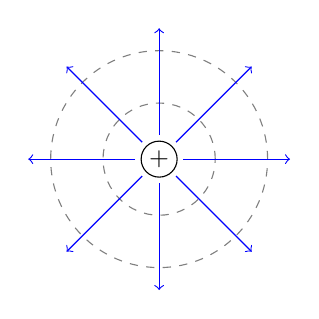
\begin{tikzpicture}[scale=0.95]
		\node[draw, circle, inner sep=0.5pt, minimum size=13pt] at (0,0) {\small $+$};
		\draw[dashed, gray] (0,0) circle (0.75);
		\draw[dashed, gray] (0,0) circle (1.45);
		\foreach \a in {0,45,...,315}
			\draw[->, blue] (\a:0.32) -- (\a:1.75);
	\end{tikzpicture}
	\hspace{1.4cm}
	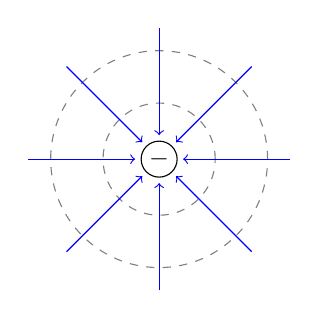
\begin{tikzpicture}[scale=0.95]
		\node[draw, circle, inner sep=0.5pt, minimum size=13pt] at (0,0) {\small $-$};
		\draw[dashed, gray] (0,0) circle (0.75);
		\draw[dashed, gray] (0,0) circle (1.45);
		\foreach \a in {0,45,...,315}
			\draw[->, blue] (\a:1.75) -- (\a:0.32);
	\end{tikzpicture}
	\end{center}

	For a dipole the lines leave the positive charge and curl round to the negative one.

	\begin{center}
	\begin{tikzpicture}[scale=1.0]
		\node[draw, circle, inner sep=0.5pt, minimum size=13pt] (P) at (-1.1,0) {\small $+$};
		\node[draw, circle, inner sep=0.5pt, minimum size=13pt] (M) at (1.1,0) {\small $-$};
		\foreach \b in {0,20,45,70} {
			\draw[blue, midarrow=0.55] (P) to[bend left=\b] (M);
			\draw[blue, midarrow=0.55] (P) to[bend right=\b] (M);
		}
		\draw[blue, midarrow=0.6] (P) to[bend right=35] (-2.5,0.85);
		\draw[blue, midarrow=0.6] (P) to[bend left=35] (-2.5,-0.85);
		\draw[blue, midarrow=0.6] (P) -- (-2.6,0);
		\draw[blue, midarrow=0.4] (2.5,0.85) to[bend left=35] (M);
		\draw[blue, midarrow=0.4] (2.5,-0.85) to[bend right=35] (M);
		\draw[blue, midarrow=0.4] (2.6,0) -- (M);
	\end{tikzpicture}
	\end{center}
\end{example}

\subsection{Electrostatic Energy}

How much energy does it take to assemble a configuration of charges? Recall from IA Dynamics and Relativity that a charge $q$ sitting at $\vv{r}$ in a potential $\phi$ has potential energy $U = q\phi(\vv{r})$; this is the work done in bringing it in from infinity, since
$$
W = -\int_\infty^{\vv{r}} \vv{F}\cdot \dd \vv{x} = -q\int_{\infty}^{\vv{r}}\vv{E}\cdot \dd \vv{x} = q\int_\infty^{\vv{r}} \nabla\phi\cdot \dd \vv{x} = q\left[\phi(\vv{r}) - \phi(\infty)\right] = q\phi(\vv{r}).
$$

Now consider $N$ point charges $q_i$ at positions $\vv{r}_i$, and build the configuration up one charge at a time. Bringing in the first costs nothing. The second must be dragged in against the field of the first, costing
$$
W_2 = \frac{1}{4\pi\epsilon_0}\frac{q_1q_2}{|\vv{r}_1-\vv{r}_2|},
$$
the third must fight both of its predecessors, and so on. Summing,
$$
U = \frac{1}{4\pi\epsilon_0}\sum_{i<j}\frac{q_iq_j}{|\vv{r}_i-\vv{r}_j|} = \frac{1}{8\pi\epsilon_0}\sum_{i\neq j}\frac{q_iq_j}{|\vv{r}_i-\vv{r}_j|},
$$
the second form counting each pair twice and compensating with a factor of $\tfrac12$. Since the potential at $\vv{r}_i$ due to all the \emph{other} charges is $\phi(\vv{r}_i) = \frac{1}{4\pi\epsilon_0}\sum_{j\neq i} q_j/|\vv{r}_i - \vv{r}_j|$, we can write this more compactly as
$$
U = \frac{1}{2}\sum_{i=1}^N q_i \phi(\vv{r}_i),
$$
which generalises to a continuous distribution as
$$
U = \frac{1}{2}\int \rho(\vv{r})\phi(\vv{r})\dd V.
$$

This is already a nice formula, but we can do better and remove the charges entirely.

\begin{proposition}[Energy in the electric field]
	\label{prop:E-energy}
	The energy of an electrostatic configuration is
	$$
	U = \frac{\epsilon_0}{2}\int_{\R^3} |\vv{E}|^2 \dd V.
	$$
\end{proposition}
\begin{proof}
	Using $\rho = \epsilon_0 \nabla \cdot \vv{E}$ and the product rule $\nabla\cdot(\phi \vv{E}) = \phi\, \nabla\cdot \vv{E} + \vv{E}\cdot\nabla\phi$,
	\begin{align*}
		U &= \frac{\epsilon_0}{2}\int (\nabla\cdot \vv{E})\phi \dd V = \frac{\epsilon_0}{2}\int \left[\nabla\cdot(\phi\vv{E}) - \vv{E}\cdot \nabla \phi\right]\dd V.
	\end{align*}
	The first term is a total divergence, so by the divergence theorem it becomes a surface integral over a sphere at infinity. For a bounded charge distribution $\phi \sim 1/r$ and $|\vv{E}| \sim 1/r^2$ while the area grows like $r^2$, so the integrand decays like $1/r$ and the term vanishes. In the second, $\nabla \phi = -\vv{E}$, leaving
	$$
	U = \frac{\epsilon_0}{2}\int \vv{E}\cdot \vv{E}\dd V. \qedhere
	$$
\end{proof}

This is a genuinely different picture of where the energy lives. The formula $U = \tfrac12 \int \rho\phi$ suggests the energy is stored `in the charges', while $U = \tfrac{\epsilon_0}{2}\int |\vv{E}|^2$ says it is stored in the field, spread out through all of space with energy density $\tfrac{\epsilon_0}{2}|\vv{E}|^2$. The second picture is the correct one, though our derivation of it from the first is not a proof of that.

\begin{remark}
	The two formulae are not quite equivalent, and it is instructive to see how they differ. For a single point charge the discrete formula gives $U = 0$ (there are no pairs), but the field is non-zero, so $\frac{\epsilon_0}{2}\int|\vv{E}|^2$ certainly is not -- indeed it diverges, since $|\vv{E}|^2 \sim r^{-4}$ near the origin. The discrepancy is the (infinite) \emph{self-energy} of the point charge, which the discrete sum quietly discards. This is the first hint of a genuine difficulty with point particles in classical field theory, and we will say no more about it here.
\end{remark}

\subsection{Conductors}

\begin{definition}[Conductor]
	A \vocab{conductor} is a region of space containing charges which are free to move.
\end{definition}

The single fact that governs everything about conductors in electrostatics is this: inside a conductor, $\vv{E} = \vv{0}$. The argument is a one-liner. If $\vv{E}$ were non-zero anywhere inside, the free charges there would feel a force and move; so we would not be in a static situation. In equilibrium the charges have rearranged themselves precisely so as to cancel the field inside. That is the whole story, and a surprising number of consequences follow from it.

\begin{proposition}[Properties of conductors]
	In electrostatic equilibrium, a conductor satisfies:
	\begin{enumerate}[label=(\roman*)]
		\item $\phi$ is constant throughout the conductor;
		\item $\rho = 0$ inside the conductor, so any net charge lives on the surface;
		\item the surface of the conductor is an equipotential, and $\vv{E}$ just outside it is perpendicular to the surface;
		\item just outside the surface, $\vv{E} = \dfrac{\sigma}{\epsilon_0}\hh{n}$, where $\sigma$ is the surface charge density and $\hh{n}$ the outward normal.
	\end{enumerate}
\end{proposition}
\begin{proof}
	(i) is immediate from $\vv{E} = -\nabla\phi = \vv{0}$. For (ii), $\rho = \epsilon_0 \nabla\cdot \vv{E} = 0$. Statement (iii) follows from (i), since the surface is part of the conductor and hence has $\phi$ constant on it, and $\vv{E}$ is normal to equipotentials. Physically, a tangential component of $\vv{E}$ at the surface would push the surface charges around. Finally (iv) is Proposition~\ref{prop:jump-E} with $\vv{E}_{\text{inside}} = \vv{0}$.
\end{proof}

Part (iv) is extremely convenient in practice: it lets us read off the induced surface charge from the field, or vice versa.

\begin{example}[Induced surface charge]
	Take a neutral spherical conductor and place it in a uniform external field, say produced by a positively charged plate on the left and a negatively charged one on the right. Far away, the field lines are straight. Near the conductor they must bend so as to meet the surface perpendicularly, and since field lines terminate on charges, there must be negative charge on the left of the sphere and positive charge on the right.

	\begin{center}
	\begin{tikzpicture}[scale=1.0]
		\draw[fill=gray!12] (0,0) circle (0.75);
		\node[anchor=east, inner sep=1pt] at (-0.15,0) {\small $-$};
		\node[anchor=west, inner sep=1pt] at (0.15,0) {\small $+$};
		\foreach \s in {-1,1} {
			\draw[blue, midarrow=0.55] (-3,\s*1.5) -- (3,\s*1.5);
		}
		\draw[blue, midarrow=0.5] (-3,0.75) to[bend left=8] (-0.6,0.45);
		\draw[blue, midarrow=0.5] (-3,-0.75) to[bend right=8] (-0.6,-0.45);
		\draw[blue, midarrow=0.5] (0.6,0.45) to[bend left=8] (3,0.75);
		\draw[blue, midarrow=0.5] (0.6,-0.45) to[bend right=8] (3,-0.75);
		\draw[blue, midarrow=0.5] (-3,0) -- (-0.75,0);
		\draw[blue, midarrow=0.5] (0.75,0) -- (3,0);
		\node[blue, anchor=south, inner sep=2pt] at (2.3,1.5) {$\vv{E}$};
	\end{tikzpicture}
	\end{center}

	The total induced charge is of course zero -- the conductor was neutral and stays so -- but it has been redistributed. This is why a conductor screens its interior: a hollow conductor (a `Faraday cage') has $\vv{E} = \vv{0}$ inside no matter what is going on outside.
\end{example}

\begin{example}[The method of images]
	Let a conductor fill the half-space $x < 0$, grounded so that $\phi = 0$ throughout it, and place a point charge $q$ at $\vv{d} = (d, 0, 0)$ with $d>0$.

	\begin{center}
	\begin{tikzpicture}[scale=1.0]
		\fill[gray!25] (-3.0,-1.75) rectangle (0,1.75);
		\draw (0,-1.75) -- (0,1.75);
		\node at (-2.1,1.15) {\small $\phi = 0$};
		\draw[fill=white] (1.7,0) circle (0.24);
		\node at (1.7,0) {\small $+$};
		\node[anchor=north, inner sep=5pt] at (1.7,-0.24) {\small $q$};
		\draw[dashed, fill=gray!25] (-1.7,0) circle (0.28);
		\node at (-1.7,0) {$-$};
		\node[anchor=north, inner sep=5pt] at (-1.7,-0.24) {\small $-q$};
		\draw[blue, midarrow=0.55] (1.44,0) -- (0.04,0);
		\draw[blue, midarrow=0.55] (1.56,0.19) to[bend left=20] (0.04,1.05);
		\draw[blue, midarrow=0.55] (1.56,-0.19) to[bend right=20] (0.04,-1.05);
		\draw[<->] (0,1.45) -- (1.7,1.45) node[midway, anchor=south, inner sep=2pt] {\small $d$};
	\end{tikzpicture}
	\end{center}

	We must solve $\nabla^2\phi = -\rho/\epsilon_0$ in $x>0$ with the boundary condition $\phi = 0$ on $x = 0$. By the uniqueness theorem, \emph{any} solution we can find is \emph{the} solution, so we are entitled to guess.

	Here is the guess. Forget the conductor and instead put an \emph{image charge} $-q$ at $(-d,0,0)$. By symmetry the potential of this pair vanishes on the plane $x = 0$, which is exactly the boundary condition we want. So we set
	$$
	\phi = \begin{cases} \dfrac{q}{4\pi \epsilon_0}\left[\dfrac{1}{|\vv{r}-\vv{d}|} - \dfrac{1}{|\vv{r}+\vv{d}|}\right] & x > 0,\\[2mm] 0 & x \leq 0.\end{cases}
	$$
	In $x>0$ this satisfies Poisson's equation with the single source at $\vv{d}$ (the image charge lies outside the region, so contributes no source there), it satisfies Laplace's equation in $x<0$, and it is continuous across $x=0$. Uniqueness does the rest.

	It remains to find the surface charge that makes this consistent. We need $E_x$ at $x = 0^+$:
	$$
	E_x = -\frac{\partial \phi}{\partial x} = \frac{q}{4\pi\epsilon_0}\left(\frac{x-d}{|\vv{r}-\vv{d}|^{3}} - \frac{x+d}{|\vv{r}+\vv{d}|^{3}}\right),
	$$
	and setting $x = 0$ gives $E_x|_{x=0} = -\dfrac{q}{2\pi \epsilon_0}\dfrac{d}{(d^2+y^2+z^2)^{3/2}}$. The outward normal of the conductor is $\hh{n} = \hh{x}$, so
	$$
	\sigma = \epsilon_0 E_x\big|_{x=0} = -\frac{q}{2\pi}\frac{d}{(d^2+y^2+z^2)^{3/2}}.
	$$
	Integrating over the plane (most easily in polar coordinates $s^2 = y^2+z^2$),
	$$
	\int \sigma \dd y \dd z = -qd\int_0^\infty \frac{s \dd s}{(d^2+s^2)^{3/2}} = -q,
	$$
	so the induced charge is exactly $-q$: every field line leaving the charge terminates on the conductor. As a byproduct, the force on the charge is the force exerted by the image, namely $q^2/16\pi\epsilon_0 d^2$ towards the plane -- a charge is always attracted to a nearby grounded conductor.
\end{example}

\begin{example}[A charge outside an earthed sphere]
	The method is not limited to planes. Take an earthed conducting sphere of radius $a$ centred at the origin, and a charge $q$ at $\vv{d}$ with $d > a$. We look for a potential vanishing on $|\vv{r}| = a$ and on the sphere's interior.

	Try a single image charge $q'$ placed at $\vv{d}' = \lambda \vv{d}$ for some $\lambda$ to be determined, so that
	$$
	\phi(\vv{r}) = \frac{1}{4\pi\epsilon_0}\left(\frac{q}{|\vv{r}-\vv{d}|} + \frac{q'}{|\vv{r}-\lambda \vv{d}|}\right).
	$$
	On the sphere $|\vv{r}| = a$, writing $\theta$ for the angle between $\vv{r}$ and $\vv{d}$,
	$$
	|\vv{r}-\vv{d}|^2 = a^2 + d^2 - 2ad\cos\theta, \qquad |\vv{r}-\lambda\vv{d}|^2 = a^2 + \lambda^2 d^2 - 2\lambda a d \cos\theta.
	$$
	For $\phi$ to vanish for \emph{all} $\theta$ we need the ratio of these to be a constant, and inspection shows that taking $\lambda = a^2/d^2$ works: then
	$$
	|\vv{r}-\lambda\vv{d}|^2 = a^2 + \frac{a^4}{d^2} - \frac{2a^3\cos\theta}{d} = \frac{a^2}{d^2}\left(d^2 + a^2 - 2ad\cos\theta\right) = \frac{a^2}{d^2}|\vv{r}-\vv{d}|^2.
	$$
	So $|\vv{r}-\lambda\vv{d}| = (a/d)|\vv{r}-\vv{d}|$ on the sphere, and $\phi = 0$ there provided
	$$
	q' = -\frac{a}{d}\,q.
	$$
	The image charge therefore sits at distance $a^2/d$ from the centre -- inside the sphere, hence outside the region where we are solving, as required -- and carries charge $-qa/d$.

	By uniqueness this is the answer. Two consequences are worth noting: the total induced charge on the sphere is $-qa/d$ (not $-q$, since the sphere is earthed and can exchange charge with the ground), and the force on $q$ is the attraction towards the image,
	$$
	F = \frac{1}{4\pi\epsilon_0}\frac{q\,|q'|}{(d - a^2/d)^2} = \frac{q^2 a d}{4\pi\epsilon_0 (d^2-a^2)^2},
	$$
	directed towards the sphere.
\end{example}

\subsection{Capacitance}

A pair of conductors carrying equal and opposite charges $\pm Q$ makes a \vocab{capacitor}. Since Poisson's equation is linear, doubling all the charges doubles all the potentials, so the potential difference $V$ between the two conductors is proportional to $Q$.

\begin{definition}[Capacitance]
	The \vocab{capacitance} of a capacitor is $C = Q/V$, where $\pm Q$ are the charges on the two conductors and $V$ is the potential difference between them. It depends only on the geometry.
\end{definition}

\begin{example}[Parallel plate capacitor]
	Take two parallel plates of area $A$, a distance $d$ apart, carrying charges $\pm Q$, and suppose $d \ll \sqrt{A}$ so we may pretend the plates are infinite and ignore what happens at the edges.

	\begin{center}
	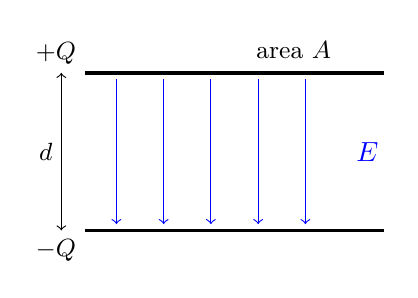
\begin{tikzpicture}[scale=1.0]
		\draw[very thick] (-1.9,1) -- (1.9,1);
		\draw[very thick] (-1.9,-1) -- (1.9,-1);
		\node[anchor=south east, inner sep=3pt] at (-1.9,1) {\small $+Q$};
		\node[anchor=north east, inner sep=3pt] at (-1.9,-1) {\small $-Q$};
		\foreach \x in {-1.5,-0.9,-0.3,0.3,0.9}
			\draw[->, blue] (\x,0.92) -- (\x,-0.92);
		\node[blue, anchor=west, inner sep=4pt] at (1.4,0) {$\vv{E}$};
		\draw[<->] (-2.2,1) -- (-2.2,-1) node[midway, anchor=east, inner sep=3pt] {\small $d$};
		\node[anchor=south, inner sep=5pt] at (0.75,1) {\small area $A$};
	\end{tikzpicture}
	\end{center}

	Each plate carries surface charge $\sigma = \pm Q/A$, and by our earlier calculation each produces a field of magnitude $\sigma/2\epsilon_0$ pointing away from the positive plate and towards the negative one. Between the plates these add; outside, they cancel. So
	$$
	\vv{E} = \frac{Q}{\epsilon_0 A}\hh{n}
	$$
	between the plates, pointing from $+$ to $-$, and $\vv{E} = \vv{0}$ outside. The potential difference is then
	$$
	V = \int \vv{E}\cdot \dd \vv{x} = \frac{Qd}{\epsilon_0 A},
	$$
	so
	$$
	C = \frac{Q}{V} = \frac{\epsilon_0 A}{d}.
	$$
	To make a large capacitance one wants large plates very close together, which is exactly what a real capacitor looks like.
\end{example}

We can also compute the energy stored, and it is a good check on Proposition~\ref{prop:E-energy}. The field occupies a volume $Ad$ and has magnitude $Q/\epsilon_0 A$, so
$$
U = \frac{\epsilon_0}{2}|\vv{E}|^2 \cdot Ad = \frac{\epsilon_0}{2}\frac{Q^2}{\epsilon_0^2A^2}Ad = \frac{Q^2 d}{2\epsilon_0 A} = \frac{Q^2}{2C} = \frac{1}{2}CV^2,
$$
which is the formula every physicist knows. Alternatively one can get it directly: to move a further charge $\dd q$ from one plate to the other against the existing potential difference $q/C$ costs $\dd W = (q/C)\dd q$, and integrating from $0$ to $Q$ gives $Q^2/2C$ again.

\begin{example}[Spherical capacitor]
	For a slightly less trivial geometry, take two concentric spherical conducting shells of radii $a < b$, the inner carrying charge $Q$ and the outer $-Q$.

	Between the shells, Gauss' law on a sphere of radius $a < r < b$ encloses charge $Q$, so
	$$
	\vv{E} = \frac{Q}{4\pi\epsilon_0 r^2}\hh{r},
	$$
	while inside the inner shell and outside the outer shell the enclosed charge is zero and $\vv{E} = \vv{0}$. The potential difference is
	$$
	V = \int_a^b \frac{Q}{4\pi \epsilon_0 r^2}\dd r = \frac{Q}{4\pi\epsilon_0}\left(\frac{1}{a}-\frac{1}{b}\right),
	$$
	so
	$$
	C = 4\pi \epsilon_0 \frac{ab}{b-a}.
	$$
	Two limits are worth noting. If $b = a + d$ with $d \ll a$, then $C \approx 4\pi\epsilon_0 a^2/d = \epsilon_0 A/d$ where $A = 4\pi a^2$: we recover the parallel plate answer, as we should, since a thin shell looks locally flat. And if we let $b\to\infty$, we get $C = 4\pi\epsilon_0 a$, the `self-capacitance' of an isolated sphere.
\end{example}

\section{Magnetostatics}

We now turn on currents and turn off time dependence. In magnetostatics we take $\rho = 0$ and $\vv{J} = \vv{J}(\vv{x})$ a steady current, and look for a time-independent magnetic field. As we noted, Maxwell's equations then reduce to
$$
\nabla \cdot \vv{B} = 0, \qquad \nabla \times \vv{B} = \mu_0 \vv{J},
$$
with $\vv{E} = \vv{0}$.

It is worth being clear about what $\rho = 0$ means here. It does \emph{not} mean there are no charges around -- we certainly need charges, or there would be no current. It means the positive and negative charges balance everywhere, and continue to do so. In a copper wire, the mobile electrons drift along while the positive ions stay put, and the two densities cancel; charge does not pile up anywhere. Mathematically, the continuity equation with $\partial \rho/\partial t = 0$ says
$$
\nabla \cdot \vv{J} = 0,
$$
which is the precise statement that current does not accumulate: whatever flows into a region flows out again. This condition is essential -- indeed, taking the divergence of $\nabla\times \vv{B} = \mu_0 \vv{J}$ forces it.

\subsection{Amp\`ere's Law}

Just as Gauss' law is the integral form of (M1), the integral form of $\nabla\times\vv{B} = \mu_0 \vv{J}$ is Amp\`ere's law. Take a surface $S$ with boundary $C = \partial S$, integrate over $S$ and apply Stokes' theorem:
$$
\oint_C \vv{B}\cdot \dd \vv{x} = \int_S(\nabla\times \vv{B})\cdot \dd \vv{S} = \mu_0 \int_S \vv{J}\cdot \dd\vv{S}.
$$

\begin{law}[Amp\`ere's law]
	For any closed curve $C$ bounding a surface $S$,
	$$
	\oint_C \vv{B}\cdot \dd \vv{x} = \mu_0 I,
	$$
	where $I$ is the total current passing through $S$, with orientations related by the right-hand rule.
\end{law}

Note that, because $\nabla\cdot\vv{J} = 0$, the current through $S$ depends only on the boundary curve $C$ and not on which surface we span it with -- a fact we will have cause to revisit when we come to the displacement current. As with Gauss' law, the utility of Amp\`ere's law lies in exploiting symmetry.

\begin{example}[The straight wire]
	Take an infinite straight wire along the $z$-axis carrying current $I$, and use cylindrical polars $(r,\varphi,z)$.

	\begin{center}
	\begin{tikzpicture}[scale=1.0]
		\draw[very thick] (0,-2.1) -- (0,1.9);
		\draw[->, very thick] (0,1.9) -- (0,2.4) node[above, inner sep=2pt] {$I$};
		\draw[blue, midarrow=0.55] (0,-1.5) ellipse (1.3 and 0.38);
		\draw[blue, midarrow=0.55] (0,0.9) ellipse (1.3 and 0.38);
		\draw[figred, thick, midarrow=0.55] (0,-0.3) ellipse (1.3 and 0.38);
		\node[figred, anchor=west, inner sep=4pt] at (1.32,-0.3) {$C$};
		\node[blue, anchor=west, inner sep=4pt] at (1.32,0.9) {$\vv{B}$};
		\draw[->] (0,-0.3) -- (1.28,-0.3) node[midway, anchor=south, inner sep=2pt] {$r$};
	\end{tikzpicture}
	\end{center}

	Symmetry under translations in $z$ and rotations about the axis says $\vv{B}$ can depend only on $r$. It can have no $z$ component (reflect in a plane perpendicular to the wire), and no radial component, since $\nabla\cdot \vv{B} = 0$ applied to a cylinder about the axis would then be violated. So
	$$
	\vv{B} = B(r)\hh{\varphi}.
	$$
	Take $C$ to be a circle of radius $r$ about the axis. Then $\dd \vv{x} = r\dd\varphi \, \hh{\varphi}$, so
	$$
	\oint_C \vv{B}\cdot \dd \vv{x} = 2\pi r B(r) = \mu_0 I,
	$$
	and hence
	$$
	\vv{B} = \frac{\mu_0 I}{2\pi r}\hh{\varphi}.
	$$
	The field circles the wire, falling off as $1/r$, with a direction given by the right-hand rule: point your right thumb along the current and your fingers curl the way $\vv{B}$ does.
\end{example}

\begin{example}[Surface current]
	Take the plane $z = 0$ to carry a \vocab{surface current density} $\vv{k}$ -- current per unit length, measured across a line in the plane perpendicular to the flow -- with $\vv{k} = k \hh{x}$.

	\begin{center}
	\begin{tikzpicture}[scale=1.0]
		\fill[gray!12] (-3.0,-0.6) -- (1.4,-0.6) -- (3.0,0.6) -- (-1.4,0.6) -- cycle;
		\draw (-3.0,-0.6) -- (1.4,-0.6) -- (3.0,0.6) -- (-1.4,0.6) -- cycle;
		\foreach \s in {-0.35,0,0.35}
			\draw[->, thick] (-2.0+\s,\s) -- (1.6+\s,\s);
		\node[anchor=north west, inner sep=2pt] at (1.95,0.35) {$\vv{k}$};
		% amperian loop
		\draw[figred, thick, midarrow=0.13] (-0.7,-1.5) -- (0.7,-1.5) -- (0.7,1.5) -- (-0.7,1.5) -- cycle;
		\node[figred, anchor=north, inner sep=4pt] at (0,-1.5) {$C$};
		\node[anchor=west, inner sep=4pt] at (0.72,1.0) {\small $L$};
	\end{tikzpicture}
	\end{center}

	Think of this as infinitely many parallel wires laid side by side. Each produces a field circling it, and adding them up, the components perpendicular to the sheet cancel in pairs while those parallel to it survive. So $\vv{B}$ points in the $\pm \hh{y}$ direction, depends only on $z$, and is odd in $z$:
	$$
	\vv{B} = -B(z)\hh{y}, \qquad B(-z) = -B(z).
	$$
	Take a rectangular loop $C$ of height $2z$ and width $L$, lying in the $y$-$z$ plane and straddling the sheet. Only the two horizontal sides contribute, and the current through the loop is $kL$, so
	$$
	\oint_C \vv{B}\cdot \dd \vv{x} = L B(z) - LB(-z) = 2LB(z) = \mu_0 k L,
	$$
	giving
	$$
	B(z) = \frac{\mu_0 k}{2} \quad \text{for } z>0.
	$$
	Once again the field is constant, and once again there is a discontinuity across the sheet -- this time in the \emph{tangential} component of $\vv{B}$. The general statement, proved by shrinking an Amp\`erian loop across an arbitrary surface exactly as in Proposition~\ref{prop:jump-E}, is
	$$
	\hh{n}\times \vv{B}_+ - \hh{n}\times\vv{B}_- = \mu_0 \vv{k},
	$$
	with the normal component of $\vv{B}$ continuous.
\end{example}

\begin{example}[The solenoid]
	A \vocab{solenoid} is a wire wound tightly into a cylindrical helix, so that it approximates a cylindrical surface current. Let there be $N$ turns per unit length, each carrying current $I$.

	\begin{center}
	\begin{tikzpicture}[scale=1.0]
		% cylinder
		\draw (0,1.9) ellipse (1.0 and 0.3);
		\draw (-1.0,1.9) -- (-1.0,-1.9);
		\draw (1.0,1.9) -- (1.0,-1.9);
		\draw[dashed] (1.0,-1.9) arc (0:180:1.0 and 0.3);
		\draw (-1.0,-1.9) arc (180:360:1.0 and 0.3);
		% windings
		\foreach \y in {-1.5,-1.0,-0.5,0,0.5,1.0,1.5} {
			\draw[figred!55, dashed] (1.0,\y) arc (0:180:1.0 and 0.3);
			\draw[figred, midarrow=0.55] (-1.0,\y) arc (180:360:1.0 and 0.3);
		}
		% B field inside
		\draw[->, blue, very thick] (0,-1.65) -- (0,1.65);
		\node[blue, anchor=west, inner sep=4pt] at (0.12,0.72) {$\vv{B}$};
		% amperian loop
		\draw[thick, midarrow=0.3] (-0.45,1.1) -- (-0.45,-1.1) -- (2.1,-1.1) -- (2.1,1.1) -- cycle;
		\node[anchor=west, inner sep=3pt] at (2.12,0.6) {$C$};
		\draw[<->] (-1.4,-1.1) -- (-1.4,1.1) node[midway, anchor=east, inner sep=3pt] {\small $L$};
		\draw[->] (3.2,-0.5) -- (3.2,0.5) node[above, inner sep=2pt] {$z$};
		\draw[->] (3.2,-0.5) -- (4.1,-0.5) node[right, inner sep=2pt] {$r$};
	\end{tikzpicture}
	\end{center}

	Symmetry (translation in $z$, rotation about the axis) together with $\nabla\cdot\vv{B} = 0$ gives $\vv{B} = B(r)\hh{z}$. Outside the solenoid there is no current, so $\nabla\times \vv{B} = \vv{0}$, and for a field of this form that says $\partial B/\partial r = 0$. So $B$ is constant outside; since it must vanish at infinity, it vanishes everywhere outside.

	Now apply Amp\`ere's law to the rectangle $C$ shown, with one vertical side of length $L$ inside the solenoid and the other outside. The outside side contributes nothing (the field is zero there) and the horizontal sides contribute nothing (they are perpendicular to $\vv{B}$, or lie where $\vv{B} = \vv{0}$). The number of wires threading the rectangle is $NL$, so
	$$
	BL = \mu_0 I N L \implies B = \mu_0 N I.
	$$
	So the field inside a solenoid is uniform, parallel to the axis, and independent of the radius. This is how one makes a uniform magnetic field in practice.
\end{example}

\subsection{The Vector Potential and Gauge}

For a general current distribution we need to deal with both equations at once, and as in electrostatics we begin by solving one of them identically. This time it is $\nabla\cdot\vv{B} = 0$, and a divergence-free field on $\R^3$ is a curl.

\begin{definition}[Vector potential]
	If $\vv{B} = \nabla \times \vv{A}$, then the vector field $\vv{A}$ is a \vocab{vector potential} for $\vv{B}$.
\end{definition}

Before going on it is worth appreciating what (M2) is telling us. In electrostatics the analogous equation was $\nabla\cdot\vv{E} = \rho/\epsilon_0$, with a source on the right. The magnetic equation has a zero there instead, and the physical content of that zero is that there are no \emph{magnetic charges}: no isolated north pole has ever been found. Break a bar magnet in half and you get two smaller magnets, never a lone north and a lone south.

Substituting $\vv{B} = \nabla\times\vv{A}$ into the remaining equation and using the identity $\nabla\times(\nabla\times \vv{A}) = \nabla(\nabla\cdot \vv{A}) - \nabla^2 \vv{A}$ gives
\begin{align*}
\nabla(\nabla\cdot \vv{A}) - \nabla^2 \vv{A} = \mu_0 \vv{J}. \tag{$*$}
\end{align*}
This looks unpleasant. What rescues us is that $\vv{A}$ is far from unique.

\begin{definition}[Gauge transformation]
	Given a vector potential $\vv{A}$ and any scalar function $\chi(\vv{x})$, the field
	$$
	\vv{A}' = \vv{A} + \nabla \chi
	$$
	is another vector potential for the same $\vv{B}$, since $\nabla\times \nabla\chi = \vv{0}$. The map $\vv{A}\mapsto \vv{A}+\nabla\chi$ is a \vocab{gauge transformation}, and a choice of $\vv{A}$ is a choice of \vocab{gauge}.
\end{definition}

So $\vv{A}$ carries redundant information: only the gauge-invariant combination $\nabla\times \vv{A}$ is physical. We may exploit this freedom to make $(*)$ as simple as possible, and the obvious thing to try is to kill the first term.

\begin{definition}[Coulomb gauge]
	A vector potential with $\nabla\cdot \vv{A} = 0$ is said to be in \vocab{Coulomb gauge}.
\end{definition}

\begin{proposition}
	Any vector potential can be brought into Coulomb gauge.
\end{proposition}
\begin{proof}
	Suppose $\nabla\cdot\vv{A} = \psi(\vv{x})$. Under a gauge transformation,
	$$
	\nabla\cdot \vv{A}' = \nabla\cdot\vv{A} + \nabla^2 \chi = \psi + \nabla^2 \chi,
	$$
	so we need $\chi$ with $\nabla^2 \chi = -\psi$. This is Poisson's equation, which we know always has a solution (write it down with the Green's function if you like). So such a $\chi$ exists.
\end{proof}

In Coulomb gauge, $(*)$ collapses to
$$
\nabla^2 \vv{A} = -\mu_0 \vv{J},
$$
or in Cartesian components, $\nabla^2 A_i = -\mu_0 J_i$: three independent copies of Poisson's equation, one for each component. We solved that in electrostatics, so we can simply write down the answer.

\begin{proposition}
	\label{prop:A-general}
	In Coulomb gauge, the vector potential of a localised steady current $\vv{J}$ is
	$$
	\vv{A}(\vv{r}) = \frac{\mu_0}{4\pi}\int \frac{\vv{J}(\vv{r}')}{|\vv{r}-\vv{r}'|}\dd V'.
	$$
\end{proposition}
\begin{proof}
	Applying the Green's function solution of Poisson's equation componentwise gives this formula, so all that remains is to check the result really is in Coulomb gauge -- otherwise it would not solve the original equation $(*)$. Taking the divergence (with $\nabla$ acting on $\vv{r}$),
	$$
	\nabla\cdot \vv{A}(\vv{r}) = \frac{\mu_0}{4\pi}\int \vv{J}(\vv{r}')\cdot \nabla\left(\frac{1}{|\vv{r}-\vv{r}'|}\right)\dd V' = -\frac{\mu_0}{4\pi}\int\vv{J}(\vv{r}')\cdot\nabla'\left(\frac{1}{|\vv{r}-\vv{r}'|}\right)\dd V',
	$$
	using the fact that differentiating $|\vv{r}-\vv{r}'|^{-1}$ with respect to $\vv{r}'$ is minus differentiating with respect to $\vv{r}$. Now that the derivative acts on the primed variable we may integrate by parts:
	$$
	\nabla \cdot \vv{A} = -\frac{\mu_0}{4\pi}\int\left[\nabla'\cdot\left(\frac{\vv{J}(\vv{r}')}{|\vv{r}-\vv{r}'|}\right) - \frac{\nabla'\cdot \vv{J}(\vv{r}')}{|\vv{r}-\vv{r}'|}\right]\dd V'.
	$$
	The first term is a total divergence, and becomes a surface integral at infinity which vanishes because the current is localised. The second vanishes because the current is steady, $\nabla'\cdot \vv{J} = 0$. So $\nabla\cdot \vv{A} = 0$.
\end{proof}

Taking the curl gives the magnetostatic analogue of the Coulomb integral.

\begin{law}[Biot--Savart law]
	The magnetic field of a localised steady current is
	$$
	\vv{B}(\vv{r}) = \frac{\mu_0}{4\pi}\int \vv{J}(\vv{r}')\times \frac{\vv{r}-\vv{r}'}{|\vv{r}-\vv{r}'|^3}\dd V'.
	$$
	If the current is confined to a thin wire along a curve $C$, then $\vv{J}\dd V' \to I \dd \vv{r}'$ and this becomes
	$$
	\vv{B}(\vv{r}) = \frac{\mu_0 I}{4\pi}\oint_C \dd \vv{r}' \times \frac{\vv{r}-\vv{r}'}{|\vv{r}-\vv{r}'|^3}.
	$$
\end{law}
\begin{proof}
	Take the curl of Proposition~\ref{prop:A-general}. Since $\nabla$ acts on $\vv{r}$ and $\vv{J}$ depends on $\vv{r}'$,
	$$
	\nabla\times\left(\frac{\vv{J}(\vv{r}')}{|\vv{r}-\vv{r}'|}\right) = \nabla\left(\frac{1}{|\vv{r}-\vv{r}'|}\right)\times \vv{J}(\vv{r}') = -\frac{\vv{r}-\vv{r}'}{|\vv{r}-\vv{r}'|^3}\times \vv{J}(\vv{r}') = \vv{J}(\vv{r}')\times\frac{\vv{r}-\vv{r}'}{|\vv{r}-\vv{r}'|^3},
	$$
	and the result follows.
\end{proof}

The Biot--Savart law is the exact analogue, for magnetostatics, of the formula $\vv{E} = \frac{1}{4\pi\epsilon_0}\int \rho (\vv{r}-\vv{r}')/|\vv{r}-\vv{r}'|^3$ we found in electrostatics -- with the cross product accounting for the fact that magnetic fields circulate rather than radiate.

\subsection{Magnetic Dipoles}

There are no magnetic monopoles, so the leading behaviour of a magnetic field far from its source is a dipole. Let us compute it.

\begin{example}[The current loop]
	Take a planar loop of wire $C$ carrying current $I$, and look at the field far away.

	\begin{center}
	\begin{tikzpicture}[scale=1.0]
		\clip (-2.7,-1.5) rectangle (2.7,1.5);
		\foreach \s in {-1,1} {
			\draw[blue] (\s*1.05,0) ellipse (0.35 and 0.5);
			\draw[blue] (\s*1.2,0) ellipse (0.72 and 1.05);
			\draw[blue] (\s*1.3,0) ellipse (1.05 and 1.9);
		}
		\draw[blue, midarrow=0.78] (0,-1.5) -- (0,1.5);
		\draw[thick, midarrow=0.8] (0,0) ellipse (1.05 and 0.45);
		\node[anchor=north east, inner sep=2pt] at (-0.72,-0.3) {\small $I$};
		\node[blue, anchor=west, inner sep=4pt] at (0.1,1.2) {$\vv{B}$};
	\end{tikzpicture}
	\end{center}

	By Proposition~\ref{prop:A-general} specialised to a wire,
	$$
	\vv{A}(\vv{r}) = \frac{\mu_0 I}{4\pi}\oint_C \frac{\dd \vv{r}'}{|\vv{r}-\vv{r}'|},
	$$
	and expanding as before,
	$$
	\vv{A}(\vv{r}) = \frac{\mu_0 I}{4\pi}\oint_C\left(\frac{1}{r} + \frac{\vv{r}\cdot \vv{r}'}{r^3}+\cdots\right)\dd \vv{r}'.
	$$
	The leading term is a constant times $\oint_C \dd \vv{r}' = \vv{0}$, so it drops out -- exactly as we should expect, since a $1/r$ term in $\vv{A}$ would be a magnetic monopole.

	For the next term we use a corollary of Stokes' theorem: for any scalar $f$,
	$$
	\oint_C f \dd \vv{r}' = \int_S \dd \vv{S}' \times \nabla' f .
	$$
	(To see this, dot both sides with a constant vector $\vv{c}$; the left becomes $\oint_C (f\vv{c})\cdot\dd\vv{r}'$, which by Stokes' theorem is $\int_S \nabla'\times(f\vv{c})\cdot\dd\vv{S}' = \int_S (\nabla' f\times \vv{c})\cdot\dd\vv{S}'$, and rearranging the triple product gives $\vv{c}\cdot\int_S \dd\vv{S}'\times\nabla' f$.)

	Taking $f(\vv{r}') = \vv{g}\cdot \vv{r}'$ for a constant vector $\vv{g}$ gives $\nabla' f = \vv{g}$, so
	$$
	\oint_C (\vv{g}\cdot \vv{r}')\dd \vv{r}' = \int_S \dd \vv{S}'\times \vv{g} = \vv{S}\times \vv{g}, \quad\text{where } \vv{S} = \int_S \dd \vv{S}'
	$$
	is the vector area of the loop. Applying this with $\vv{g} = \vv{r}/r^3$,
	$$
	\vv{A}(\vv{r}) \approx \frac{\mu_0}{4\pi}\frac{\vv{m}\times \vv{r}}{r^3},
	$$
	where we have defined the following.
	\begin{definition}[Magnetic dipole moment]
		The \vocab{magnetic dipole moment} of a current loop is $\vv{m} = I \vv{S}$, with $\vv{S}$ the vector area of the loop.
	\end{definition}
	Taking the curl (a slightly tedious but routine index computation) gives
	$$
	\vv{B} = \nabla\times \vv{A} = \frac{\mu_0}{4\pi}\left(\frac{3(\vv{m}\cdot\hh{r})\hh{r} - \vv{m}}{r^3}\right),
	$$
	which is precisely the same shape as the electric field of an electric dipole, with $\vv{p}/\epsilon_0$ replaced by $\mu_0 \vv{m}$. The difference is that the magnetic expansion has no $1/r^2$ monopole term at all.
\end{example}

The same conclusion holds for an arbitrary localised current, though the computation takes a little more care.

\begin{proposition}[Dipole moment of a general current]
	For a localised steady current $\vv{J}$,
	$$
	\vv{A}(\vv{r}) = \frac{\mu_0}{4\pi}\frac{\vv{m}\times \vv{r}}{r^3} + O(r^{-3}), \qquad \vv{m} = \frac{1}{2}\int \vv{r}'\times \vv{J}(\vv{r}')\dd V'.
	$$
\end{proposition}
\begin{proof}
	Expanding Proposition~\ref{prop:A-general} in components,
	$$
	A_i(\vv{r}) = \frac{\mu_0}{4\pi}\int\left(\frac{J_i(\vv{r}')}{r} + \frac{J_i(\vv{r}')(\vv{r}\cdot \vv{r}')}{r^3}+\cdots\right)\dd V'.
	$$
	For the first term, note that since $\partial_j' J_j = \nabla'\cdot \vv{J} = 0$ and $\partial_j' r_i' = \delta_{ij}$,
	$$
	\partial_j'(J_j r_i') = (\partial_j'J_j)r_i' + J_j \delta_{ij} = J_i,
	$$
	so $J_i$ is a total derivative and its integral vanishes.

	For the second, apply the same trick to $J_j r_i'r_k'$:
	$$
	\partial_j'(J_j r_i' r_k') = J_i r_k' + J_k r_i',
	$$
	so the symmetric part of $J_ir_k'$ integrates to zero, and only the antisymmetric part survives:
	$$
	\int J_i (\vv{r}\cdot\vv{r}')\dd V' = \int \frac{r_k}{2}\left(J_ir_k' - J_kr_i'\right)\dd V' = \frac{1}{2}\int \left[\vv{r}\times(\vv{J}\times\vv{r}')\right]_i \dd V'.
	$$
	Rearranging the triple product and comparing with $(\vv{m}\times \vv{r})_i$ gives the result with the stated $\vv{m}$.
\end{proof}

For a planar loop the two definitions agree: $\frac{1}{2}\oint \vv{r}'\times I\dd \vv{r}'$ is $I$ times the vector area, which is $I\vv{S}$.

\subsection{Magnetic Forces}

Currents make magnetic fields, and magnetic fields push currents. Hence currents push each other. The relevant formula is the continuum Lorentz force law from Section~1,
$$
\vv{F} = \int \vv{J}\times \vv{B}\dd V,
$$
which for a thin wire becomes $\vv{F} = I\oint_C \dd \vv{r}\times \vv{B}$.

\begin{example}[Force between parallel wires]
	Take two infinite parallel wires a distance $d$ apart, carrying currents $I_1$ and $I_2$ in the same direction, say along $\hh{z}$, and separated along $\hh{x}$.

	\begin{center}
	\begin{tikzpicture}[scale=1.0]
		\draw[thick, midarrow=0.55] (-1.4,-1.7) -- (-1.4,2.0);
		\draw[thick, midarrow=0.55] (1.4,-1.7) -- (1.4,2.0);
		\node[anchor=south, inner sep=3pt] at (-1.4,2.0) {$I_1$};
		\node[anchor=south, inner sep=3pt] at (1.4,2.0) {$I_2$};
		\draw[<->] (-1.4,-1.4) -- (1.4,-1.4) node[midway, anchor=south, inner sep=3pt] {$d$};
		\draw[->, figred, thick] (-1.36,0.95) -- (-0.5,0.95);
		\draw[->, figred, thick] (1.36,0.95) -- (0.5,0.95);
		\node[figred, anchor=south, inner sep=4pt] at (0,0.95) {\small attraction};
		\draw[blue] (0.9,-0.45) circle (0.17);
		\draw[blue] (0.78,-0.57) -- (1.02,-0.33);
		\draw[blue] (0.78,-0.33) -- (1.02,-0.57);
		\node[blue, anchor=east, inner sep=4pt] at (0.71,-0.45) {$\vv{B}_1$};
	\end{tikzpicture}
	\end{center}

	The first wire produces at the location of the second a field of magnitude
	$$
	B_1 = \frac{\mu_0 I_1}{2\pi d},
	$$
	pointing in the $\hh{\varphi}$ direction, which at the second wire is $-\hh{y}$ (taking the wires along $\hh{z}$ separated in $\hh{x}$). The force per unit length on the second wire is then
	$$
	\frac{\vv{F}}{L} = I_2 \hh{z}\times \vv{B}_1 = -\frac{\mu_0 I_1I_2}{2\pi d}\,\hh{z}\times\hh{y} = \frac{\mu_0 I_1I_2}{2\pi d}\hh{x},
	$$
	which points from the second wire towards the first. So parallel currents \emph{attract}, and (reversing $I_2$) antiparallel currents repel. This is exactly backwards from the electrostatic case, where like charges repel, and it is the reason the definition of the Ampere used to be phrased in terms of the force between two wires.
\end{example}

\begin{example}[General force between current loops]
	More generally, a current $I_1$ on a loop $C_1$ produces, by Biot--Savart,
	$$
	\vv{B}(\vv{r}) = \frac{\mu_0 I_1}{4\pi}\oint_{C_1}\dd \vv{r}_1 \times \frac{\vv{r}-\vv{r}_1}{|\vv{r}-\vv{r}_1|^3},
	$$
	and a second loop $C_2$ carrying $I_2$ then feels
	$$
	\vv{F} = \frac{\mu_0 I_1I_2}{4\pi}\oint_{C_2}\oint_{C_1}\dd \vv{r}_2 \times \left(\dd \vv{r}_1 \times \frac{\vv{r}_2-\vv{r}_1}{|\vv{r}_2-\vv{r}_1|^3}\right).
	$$
	This double integral is not something one wants to evaluate. If the loops are far apart, though, each looks like a dipole, and the force can be shown to be
	$$
	\vv{F} = \frac{\mu_0}{4\pi}\nabla\left(\frac{3(\vv{m}_1\cdot\hh{r})(\vv{m}_2\cdot\hh{r}) - \vv{m}_1\cdot\vv{m}_2}{r^3}\right),
	$$
	the gradient of an interaction energy of exactly the same form as for two electric dipoles. We omit the (long) proof.
\end{example}

There is one more result worth recording, on a small current loop placed in an \emph{external} field. It is the exact magnetic analogue of Proposition~\ref{prop:dipole-external}.

\begin{proposition}[Magnetic dipole in an external field]
	A small current loop of dipole moment $\vv{m}$ in an external field $\vv{B}$ experiences a torque
	$$
	\vv{\tau} = \vv{m}\times\vv{B},
	$$
	and has interaction energy $U = -\vv{m}\cdot\vv{B}$, so that in a non-uniform field it feels a force $\vv{F} = \nabla(\vv{m}\cdot\vv{B})$.
\end{proposition}
\begin{proof}
	If $\vv{B}$ is essentially constant over the loop, the net force is
	$$
	\vv{F} = I\oint_C \dd \vv{r}\times \vv{B} = I\left(\oint_C \dd \vv{r}\right)\times\vv{B} = \vv{0},
	$$
	since the integral of $\dd\vv{r}$ round a closed curve vanishes. The torque about the centre of the loop is
	$$
	\vv{\tau} = I\oint_C \vv{r}\times(\dd \vv{r}\times \vv{B}) = I\oint_C\left[\dd \vv{r}\,(\vv{r}\cdot\vv{B}) - \vv{B}\,(\vv{r}\cdot\dd\vv{r})\right],
	$$
	by the vector triple product. The second term vanishes, since $\oint_C \vv{r}\cdot\dd\vv{r} = \oint_C \dd(\tfrac12 r^2) = 0$. For the first, apply the identity $\oint_C(\vv{g}\cdot\vv{r})\dd\vv{r} = \vv{S}\times\vv{g}$ established in the current loop example, with $\vv{g} = \vv{B}$:
	$$
	\vv{\tau} = I\,\vv{S}\times \vv{B} = \vv{m}\times\vv{B},
	$$
	as claimed. Finally, $U = -\vv{m}\cdot\vv{B}$ is the energy function whose angular derivative reproduces this torque, and whose spatial gradient gives the force.
\end{proof}

This is why a compass needle turns to point along the field, and why an electric motor turns: a current loop in a magnetic field twists until its moment aligns, and if you flip the current at the right moment it keeps twisting. A bar magnet is, at bottom, an enormous number of microscopic current loops -- electron spins, really -- whose dipole moments have lined up, and the force $\nabla(\vv{m}\cdot\vv{B})$ is what makes it stick to a fridge.

We have now spent a whole section on `magnets' which look nothing at all like the ones in a kitchen drawer. The bridge between the two is the observation just made, and the details belong to a course on the electromagnetism of media.

\section{Electrodynamics}

We now allow the fields to depend on time, and the two halves of the theory become inseparable. A changing magnetic field produces an electric field, and a changing electric field produces a magnetic field; put the two together and you get a self-sustaining disturbance which propagates through empty space at the speed of light.

\subsection{Induction and Faraday's Law}

We begin with the Maxwell equation we have so far ignored,
$$
\nabla \times \vv{E} + \frac{\partial \vv{B}}{\partial t} = \vv{0}.
$$
Integrate it over a fixed surface $S$ with boundary $C$, and apply Stokes' theorem:
$$
\oint_C \vv{E}\cdot \dd \vv{x} = -\int_S \frac{\partial \vv{B}}{\partial t}\cdot \dd \vv{S} = -\frac{\dd}{\dd t}\int_S \vv{B}\cdot \dd \vv{S},
$$
the last step being legitimate because $S$ is not moving. Both sides deserve names.

\begin{definition}[Electromotive force and magnetic flux]
	The \vocab{electromotive force} (emf) around a closed curve $C$ is
	$$
	\mathcal{E} = \oint_C \vv{E}\cdot \dd \vv{x},
	$$
	and the \vocab{magnetic flux} through a surface $S$ is
	$$
	\Phi = \int_S \vv{B}\cdot \dd \vv{S}.
	$$
\end{definition}

The name `electromotive force' is a historical embarrassment: $\mathcal{E}$ is not a force but a work done per unit charge, and it is measured in volts. If $C$ is a loop of wire, $\mathcal{E}$ is the voltage that the loop sees.

\begin{law}[Faraday's law of induction]
	$$
	\mathcal{E} = -\frac{\dd \Phi}{\dd t}.
	$$
\end{law}

So changing the flux through a circuit drives a current around it. There are many ways to change the flux -- move a magnet towards the loop, switch an electromagnet on or off, rotate the loop -- and all of them work. Essentially every electrical generator in the world runs on this principle.

The minus sign is worth dwelling on. It says that the induced current flows in the direction whose own magnetic field \emph{opposes} the change in flux. This is \vocab{Lenz's law}, and it is a statement about stability: were the sign the other way, an increase in flux would induce a current reinforcing the increase, which would induce more current, and so on. The world would rapidly become unpleasant.

\begin{example}[A loop in a decreasing field]
	Consider a circular loop of wire with a magnetic field passing up through it, and suppose we decrease $|\vv{B}|$.

	\begin{center}
	\begin{tikzpicture}[scale=1.0]
		\fill[gray!12] (0,0) ellipse (1.7 and 0.55);
		\foreach \x in {-1.1,-0.55,0,0.55,1.1}
			\draw[->, blue] (\x,-1.0) -- (\x,1.3);
		\draw[figred, thick, midarrow=0.28] (0,0) ellipse (1.7 and 0.55);
		\node[figred, anchor=east, inner sep=4pt] at (-1.72,0) {$I$};
		\node[anchor=west, inner sep=4pt] at (1.72,0) {$S$};
		\node[blue, anchor=south, inner sep=3pt] at (1.1,1.3) {$\vv{B}$};
	\end{tikzpicture}
	\end{center}

	Then $\dd \Phi/\dd t < 0$, so $\mathcal{E} > 0$ and the current flows anticlockwise when viewed from above. By the right-hand rule this current produces a magnetic field pointing \emph{up} through the loop, which is to say it tries to maintain the flux that we are removing. Lenz's law in action.
\end{example}

There is a second, superficially quite different, way to change the flux: keep $\vv{B}$ fixed and move the circuit. Remarkably, the same formula holds.

\begin{example}[The sliding bar]
	Take a conducting bar of length $d$ sliding with speed $v$ along a pair of rails, in a uniform field $\vv{B}$ perpendicular to the plane of the circuit.

	\begin{center}
	\begin{tikzpicture}[scale=1.0]
		% rails (parallelogram region)
		\fill[gray!10] (0,0) -- (4.2,0) -- (5.0,1.3) -- (0.8,1.3) -- cycle;
		\draw (0,0) -- (4.2,0);
		\draw (0.8,1.3) -- (5.0,1.3);
		\draw (0,0) -- (0.8,1.3);
		% sliding bar
		\draw[very thick] (2.1,-0.25) -- (3.05,1.55);
		\node[anchor=east, inner sep=3pt] at (0.32,0.72) {$d$};
		\draw[->, figred, thick] (2.2,-0.6) -- (1.3,-0.6);
		\node[figred, anchor=east, inner sep=3pt] at (1.28,-0.6) {$\vv{v}$};
		\foreach \x in {1.1,1.7,3.4,4.0}
			\draw[->, blue] (\x,0.4) -- (\x,1.95);
		\node[blue, anchor=south, inner sep=3pt] at (4.0,1.95) {$\vv{B}$};
	\end{tikzpicture}
	\end{center}

	Here nothing is changing in time at any fixed point of space, so the Maxwell equation we used above has nothing to say. Instead, use the Lorentz force law directly: each charge $q$ in the bar is being carried along at velocity $\vv{v}$, so it feels a force $q\vv{v}\times\vv{B}$ of magnitude $qvB$ directed along the bar. The work done per unit charge in going once round the circuit is therefore
	$$
	\mathcal{E} = vBd,
	$$
	since only the charges in the moving bar have any force on them. Meanwhile the area of the circuit is shrinking at rate $vd$, so
	$$
	\frac{\dd \Phi}{\dd t} = -vBd,
	$$
	and once again $\mathcal{E} = -\dd \Phi/\dd t$. The same law, but for a completely different reason -- one is Maxwell's equation, the other is the Lorentz force law. That these two conspire to give the same answer is a strong hint that something deeper is going on, and in Section~\ref{sec:relativity} we will see what.
\end{example}

Let us do the general case, in which both effects occur at once.

\begin{theorem}[The flux rule]
	Let $C(t)$ be a moving closed curve bounding a moving surface $S(t)$, with the curve moving with local velocity $\vv{v}$. Define the emf as
	$$
	\mathcal{E} = \oint_{C(t)} (\vv{E} + \vv{v}\times \vv{B})\cdot \dd \vv{x}.
	$$
	Then $\mathcal{E} = -\dd \Phi/\dd t$.
\end{theorem}
\begin{proof}
	As the curve moves from time $t$ to $t+\delta t$, it sweeps out a cylindrical surface $S_c$, and $S(t)$, $S(t+\delta t)$ and $S_c$ together bound a volume.

	\begin{center}
	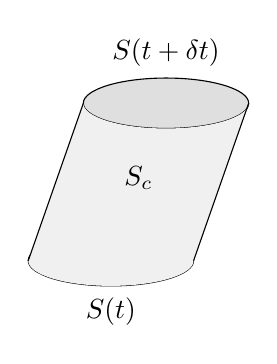
\begin{tikzpicture}[scale=1.0]
		\fill[gray!25] (0,0) ellipse (1.05 and 0.32);
		\draw (0,0) ellipse (1.05 and 0.32);
		\node[anchor=north, inner sep=4pt] at (0,-0.32) {$S(t)$};
		\fill[gray!25] (0.7,2) ellipse (1.05 and 0.32);
		\draw (0.7,2) ellipse (1.05 and 0.32);
		\node[anchor=south, inner sep=4pt] at (0.7,2.32) {$S(t+\delta t)$};
		\fill[gray!12] (-1.05,0) -- (-0.35,2) arc (180:360:1.05 and 0.32) -- (1.05,0) arc (0:-180:1.05 and 0.32);
		\draw (-1.05,0) -- (-0.35,2);
		\draw (1.05,0) -- (1.75,2);
		\node at (0.35,1.05) {$S_c$};
	\end{tikzpicture}
	\end{center}

	Now compute the change in flux, expanding $\vv{B}(t+\delta t) = \vv{B}(t) + \delta t \, \partial\vv{B}/\partial t + O(\delta t^2)$:
	\begin{align*}
		\Phi(t+\delta t) - \Phi(t) &= \int_{S(t+\delta t)}\vv{B}(t+\delta t)\cdot \dd \vv{S} - \int_{S(t)}\vv{B}(t)\cdot \dd \vv{S}\\
		&= \delta t \int_{S(t)}\frac{\partial \vv{B}}{\partial t}\cdot\dd\vv{S} + \left[\int_{S(t+\delta t)} - \int_{S(t)}\right]\vv{B}(t)\cdot \dd\vv{S} + O(\delta t^2).
	\end{align*}
	Since $\nabla\cdot\vv{B} = 0$, the flux of $\vv{B}(t)$ out of the closed surface formed by $S(t+\delta t)$, $S(t)$ and $S_c$ is zero, which says exactly
	$$
	\left[\int_{S(t+\delta t)} - \int_{S(t)}\right]\vv{B}(t)\cdot \dd \vv{S} = -\int_{S_c}\vv{B}(t)\cdot \dd \vv{S}.
	$$
	On $S_c$, an element of the curve $\dd \vv{x}$ sweeps out area $\dd \vv{S} = \dd \vv{x}\times \vv{v}\,\delta t$, so $\vv{B}\cdot \dd \vv{S} = \delta t\,(\vv{v}\times \vv{B})\cdot \dd \vv{x}$. Dividing by $\delta t$ and letting $\delta t \to 0$,
	$$
	\frac{\dd \Phi}{\dd t} = \int_{S(t)}\frac{\partial \vv{B}}{\partial t}\cdot \dd\vv{S} - \oint_{C(t)}(\vv{v}\times \vv{B})\cdot \dd \vv{x}.
	$$
	Finally substitute $\partial\vv{B}/\partial t = -\nabla\times \vv{E}$ from (M3) and apply Stokes' theorem to the first term:
	$$
	\frac{\dd \Phi}{\dd t} = -\oint_{C(t)}\vv{E}\cdot \dd \vv{x} - \oint_{C(t)}(\vv{v}\times \vv{B})\cdot \dd\vv{x} = -\mathcal{E}. \qedhere
	$$
\end{proof}

So the two mechanisms are two terms of one formula, and the flux rule is completely general.

\subsection{Inductance and Magnetic Energy}

Consider a loop of wire $C$ carrying current $I$. This produces a magnetic field, and hence a flux through the loop itself. By linearity, the flux is proportional to the current.

\begin{definition}[Inductance]
	The \vocab{inductance} of a circuit $C$ is $L = \Phi/I$, the flux through $C$ per unit current flowing in $C$. It depends only on the geometry of $C$.
\end{definition}

\begin{example}[Inductance of a solenoid]
	Take a solenoid of length $\ell$ and cross-sectional area $A$, with $N$ turns per unit length, and suppose $\ell \gg \sqrt{A}$ so that we may use $B = \mu_0 N I$ throughout. The flux through a single turn is $\Phi_0 = \mu_0 N I A$, and there are $N\ell$ turns in total, so
	$$
	\Phi = \mu_0 N^2 I A \ell = \mu_0 N^2 I V,
	$$
	where $V = A\ell$ is the volume. Hence
	$$
	L = \mu_0 N^2 V.
	$$
\end{example}

There is also a version of this for two circuits, which is what makes transformers possible.

\begin{definition}[Mutual inductance]
	Given two circuits $C_1$ and $C_2$, the \vocab{mutual inductance} $M$ is defined by $\Phi_2 = M I_1$, where $\Phi_2$ is the flux through $C_2$ produced by a current $I_1$ in $C_1$.
\end{definition}

It is a small miracle -- and a very useful one -- that $M$ is symmetric in the two circuits.

\begin{proposition}
	The flux through $C_2$ due to unit current in $C_1$ equals the flux through $C_1$ due to unit current in $C_2$.
\end{proposition}
\begin{proof}
	Using $\vv{B} = \nabla\times\vv{A}$, Stokes' theorem, and the expression for the vector potential of a wire,
	$$
	\Phi_2 = \int_{S_2}\vv{B}_1\cdot\dd\vv{S} = \oint_{C_2}\vv{A}_1\cdot \dd\vv{r}_2 = \frac{\mu_0 I_1}{4\pi}\oint_{C_2}\oint_{C_1}\frac{\dd \vv{r}_1\cdot \dd\vv{r}_2}{|\vv{r}_1-\vv{r}_2|}.
	$$
	The right hand side is manifestly symmetric under exchanging the roles of $C_1$ and $C_2$, so $M$ is too. (This is the \vocab{Neumann formula}.)
\end{proof}

Inductance is the key to computing the energy stored in a magnetic field, by the following argument. To build up a current we must change it, and by Faraday's law a changing current induces an emf
$$
\mathcal{E} = -\frac{\dd \Phi}{\dd t} = -L\frac{\dd I}{\dd t}
$$
which, by Lenz's law, opposes what we are trying to do. So we must do work against it. In a time $\delta t$ a charge $I\delta t$ goes round the loop, and the work we must do against the induced emf is
$$
\delta W = -\mathcal{E} I\, \delta t = LI \frac{\dd I}{\dd t}\delta t = \frac{L}{2}\frac{\dd (I^2)}{\dd t}\delta t.
$$
Integrating from zero current up to $I$,
$$
W = \frac{1}{2}LI^2 = \frac{1}{2}I\Phi.
$$

\begin{proposition}[Energy in the magnetic field]
	\label{prop:B-energy}
	The energy stored in a magnetic field is
	$$
	U = \frac{1}{2\mu_0}\int_{\R^3}|\vv{B}|^2 \dd V.
	$$
\end{proposition}
\begin{proof}
	Start from $U = \tfrac12 I \Phi$, write $\vv{B} = \nabla\times\vv{A}$ and use Stokes' theorem:
	\begin{align*}
		U &= \frac{1}{2}I\int_S \vv{B}\cdot \dd \vv{S} = \frac{1}{2}I\int_S (\nabla\times \vv{A})\cdot \dd \vv{S} = \frac{1}{2}I\oint_C \vv{A}\cdot\dd\vv{x} = \frac{1}{2}\int_{\R^3}\vv{J}\cdot \vv{A}\dd V,
	\end{align*}
	the last step because the current is confined to the wire, where $\vv{J}\dd V = I \dd \vv{x}$. Now use $\vv{J} = (\nabla\times\vv{B})/\mu_0$ and the identity $\nabla\cdot(\vv{B}\times\vv{A}) = \vv{A}\cdot(\nabla\times\vv{B}) - \vv{B}\cdot(\nabla\times\vv{A})$:
	\begin{align*}
		U &= \frac{1}{2\mu_0}\int (\nabla\times \vv{B})\cdot \vv{A}\dd V = \frac{1}{2\mu_0}\int\left[\nabla\cdot(\vv{B}\times\vv{A}) + \vv{B}\cdot(\nabla\times\vv{A})\right]\dd V.
	\end{align*}
	The first term is a total divergence and integrates to a surface term at infinity, which vanishes provided $\vv{B}\times\vv{A}$ decays fast enough. The second is $|\vv{B}|^2$, giving the result.
\end{proof}

Comparing with Proposition~\ref{prop:E-energy}, the total energy stored in the electromagnetic field is
$$
U = \int_{\R^3}\left(\frac{\epsilon_0}{2}|\vv{E}|^2 + \frac{1}{2\mu_0}|\vv{B}|^2\right)\dd V.
$$
It is worth flagging that this does not follow logically from the two separate results: in principle, when both fields are present, they might interact and contribute cross terms $\vv{E}\cdot\vv{B}$ to the energy. They do not, but seeing why requires the Poynting theorem, which we prove below.

\subsection{Resistance and Circuits}

So far our story is: change the flux, get an emf, accelerate the charges. But charges that accelerate forever would give infinite currents, and in reality they do not. What stops them is a form of friction: the charges collide with the atoms of the wire, losing energy. The upshot is that the emf ends up proportional to the charges' \emph{velocity} rather than their acceleration.

\begin{law}[Ohm's law]
	For most materials, the current is proportional to the applied emf:
	$$
	\mathcal{E} = IR,
	$$
	where $R$ is the \vocab{resistance} of the circuit. In terms of fields, this reads $\vv{J} = \sigma \vv{E}$, where $\sigma$ is the \vocab{conductivity} of the material.
\end{law}

Since $\mathcal{E} = \oint \vv{E}\cdot \dd \vv{x}$ is the potential difference $V$ in the static case, this is the familiar $V = IR$. For a wire of length $\ell$ and cross-section $A$ made of a material of \vocab{resistivity} $\varrho = 1/\sigma$, one finds $R = \varrho \ell /A$; the resistivity is a property of the substance alone, while the resistance depends on the shape.

Resistance costs energy. In time $\delta t$ a charge $I\delta t$ moves round the circuit through a potential difference $\mathcal{E}$, so
$$
\frac{\dd W}{\dd t} = \mathcal{E}I = I^2 R.
$$
This is \vocab{Joule heating}: the energy lost to the collisions, which reappears as heat. It is how an electric kettle works, and why a computer needs a fan.

\begin{example}[The decelerating bar]
	Return to the sliding bar, and now give the bar resistance $R$ (taking the rails to be perfect conductors).

	\begin{center}
	\begin{tikzpicture}[scale=1.0]
		\fill[gray!10] (0,0) -- (4.2,0) -- (5.0,1.3) -- (0.8,1.3) -- cycle;
		\draw (0,0) -- (4.2,0);
		\draw (0.8,1.3) -- (5.0,1.3);
		\draw (0,0) -- (0.8,1.3);
		\draw[very thick] (2.1,-0.25) -- (3.05,1.55);
		\node[anchor=west, inner sep=5pt] at (2.72,0.55) {\small $R$};
		\node[anchor=east, inner sep=3pt] at (0.32,0.72) {$\ell$};
		\draw[->, figred, thick] (2.2,-0.6) -- (1.3,-0.6);
		\node[figred, anchor=east, inner sep=3pt] at (1.28,-0.6) {$\vv{v}$};
		\foreach \x in {1.1,1.7,3.4,4.0}
			\draw[->, blue] (\x,0.4) -- (\x,1.95);
		\node[blue, anchor=south, inner sep=3pt] at (4.0,1.95) {$\vv{B}$};
	\end{tikzpicture}
	\end{center}

	There are two unknowns: the position $x(t)$ of the bar and the current $I(t)$. A current $I$ in the bar feels a force $I\ell B$ along the rails, so
	$$
	m\ddot x = I B\ell.
	$$
	Meanwhile the emf is $\mathcal{E} = -\dd\Phi/\dd t = -B\ell \dot x$, so Ohm's law gives $IR = -B\ell\dot x$. Eliminating $I$,
	$$
	m\ddot x = -\frac{B^2\ell^2}{R}\dot x,
	$$
	which integrates to
	$$
	\dot x(t) = -v\, e^{-B^2\ell^2 t/mR}.
	$$
	The bar decelerates exponentially. This is Lenz's law again -- the induced current opposes the motion that produced it -- and its kinetic energy is dissipated as Joule heating in the bar. It is exactly the mechanism behind magnetic braking.
\end{example}

\begin{example}[The LR circuit]
	Put an inductor $L$, a resistor $R$ and a battery of emf $\mathcal{E}_0$ in series, and close the switch at $t = 0$.

	\begin{center}
	\begin{tikzpicture}[scale=1.0]
		% wires
		\draw (0,1.6) -- (1.0,1.6);
		\draw (2.4,1.6) -- (3.6,1.6) -- (3.6,0) -- (2.2,0);
		\draw (1.4,0) -- (0,0);
		\draw (0,0) -- (0,0.7);
		\draw (0,0.95) -- (0,1.6);
		% inductor coils
		\foreach \i in {0,1,2,3} {
			\draw (1.0+0.35*\i,1.6) arc (180:0:0.175);
		}
		\node[anchor=south, inner sep=7pt] at (1.7,1.72) {$L$};
		% resistor
		\draw (1.4,-0.18) rectangle (2.2,0.18);
		\node[anchor=north, inner sep=6pt] at (1.8,-0.18) {$R$};
		% battery
		\draw (-0.22,0.95) -- (0.22,0.95);
		\draw (-0.1,0.7) -- (0.1,0.7);
		\node[anchor=east, inner sep=8pt] at (0,0.82) {$\mathcal{E}_0$};
		% current
		\draw[->, figred, thick] (2.6,1.85) -- (3.25,1.85);
		\node[figred, anchor=south, inner sep=3pt] at (2.92,1.85) {$I$};
	\end{tikzpicture}
	\end{center}

	Going round the loop, the battery supplies $\mathcal{E}_0$, the inductor opposes with $-L\dd I/\dd t$, and the resistor drops $IR$:
	$$
	\mathcal{E}_0 - L\frac{\dd I}{\dd t} = IR.
	$$
	This is a first order linear ODE with solution
	$$
	I(t) = \frac{\mathcal{E}_0}{R}\left(1 - e^{-Rt/L}\right),
	$$
	so the current does not jump to its final value $\mathcal{E}_0/R$ instantly but rises on a timescale $L/R$. Inductors resist changes in current, in exactly the way that masses resist changes in velocity.
\end{example}

\subsection{The Displacement Current}
\label{sec:displacement}

We have now used every one of Maxwell's equations except for the final term in (M4),
$$
\nabla\times \vv{B} = \mu_0\left(\vv{J} + \epsilon_0 \frac{\partial \vv{E}}{\partial t}\right),
$$
in which the quantity $\epsilon_0 \partial \vv{E}/\partial t$ is called, for historical reasons, the \vocab{displacement current}. It is the smallest looking term in Maxwell's equations and by far the most consequential.

Its necessity is a matter of pure mathematics, and was noticed as such. Suppose we drop it, as Amp\`ere did, and write $\nabla\times \vv{B} = \mu_0\vv{J}$. Taking the divergence, and using that the divergence of a curl vanishes,
$$
\mu_0 \nabla\cdot \vv{J} = \nabla\cdot(\nabla\times\vv{B}) = 0.
$$
But charge conservation says $\dot \rho + \nabla\cdot \vv{J} = 0$, so this forces $\dot\rho = 0$ everywhere and always. That is absurd -- we can perfectly well pick up a charge and carry it somewhere else, changing $\rho$ as we go. So the equations as they stood were inconsistent with the conservation of charge.

With the extra term the computation instead reads
$$
0 = \nabla\cdot\left(\vv{J} + \epsilon_0\frac{\partial \vv{E}}{\partial t}\right) = \nabla\cdot\vv{J} + \epsilon_0\frac{\partial}{\partial t}(\nabla\cdot\vv{E}) = \nabla\cdot \vv{J} + \frac{\partial \rho}{\partial t},
$$
using (M1). So not only is the theory now consistent with charge conservation, it \emph{implies} it. This is a beautiful piece of physics: Maxwell found the term by demanding mathematical consistency, and it turned out to predict light.

\begin{example}[The charging capacitor]
	Here is the standard illustration of why the term is needed. Take a wire carrying current $I$ into one plate of a capacitor, and consider Amp\`ere's law on a circle $C$ around the wire. We may span $C$ with a flat disc $S_1$ cut by the wire, or with a bulging surface $S_2$ that passes between the plates.

	\begin{center}
	\begin{tikzpicture}[scale=1.0]
		\draw[thick] (-4.0,0) -- (-0.7,0);
		\draw[thick] (0.7,0) -- (3.2,0);
		\draw[->, thick] (-3.6,0) -- (-3.15,0);
		\node[anchor=south, inner sep=4pt] at (-3.4,0) {$I$};
		\draw[very thick] (-0.7,-1.0) -- (-0.7,1.0);
		\draw[very thick] (0.7,-1.0) -- (0.7,1.0);
		% loop C, and the flat surface S1
		\fill[gray!25] (-2.4,0) ellipse (0.26 and 1.15);
		\draw[figred, thick] (-2.4,0) ellipse (0.26 and 1.15);
		\node[figred, anchor=south, inner sep=3pt] at (-2.4,1.15) {$C$};
		\node[anchor=east, inner sep=5pt] at (-2.66,-0.6) {$S_1$};
		% S2
		\draw[blue, dashed] (-2.4,1.15) .. controls (-1.6,1.9) and (0.3,1.7) .. (0.0,0.0)
			.. controls (0.3,-1.7) and (-1.6,-1.9) .. (-2.4,-1.15);
		\node[blue, anchor=south, inner sep=3pt] at (-1.0,1.65) {$S_2$};
		% field in the gap
		\foreach \y in {-0.75,-0.35,0.35,0.75}
			\draw[->, blue] (-0.65,\y) -- (0.65,\y);
		\node[blue, anchor=south, inner sep=4pt] at (0,1.02) {$\vv{E}$};
	\end{tikzpicture}
	\end{center}

	Through $S_1$ the current is $I$; through $S_2$ it is zero, since no charge crosses the gap. Without the displacement current Amp\`ere's law would give two different answers, which is not acceptable. With it, we note that the charge $Q$ on the plate gives a field $E = Q/\epsilon_0 A$ in the gap, so the displacement current through $S_2$ is
	$$
	\epsilon_0 \frac{\dd}{\dd t}\int_{S_2}\vv{E}\cdot\dd\vv{S} = \epsilon_0 A \frac{\dd}{\dd t}\left(\frac{Q}{\epsilon_0 A}\right) = \frac{\dd Q}{\dd t} = I,
	$$
	exactly making up the difference. The two surfaces agree, as they must.
\end{example}

\subsection{Electromagnetic Waves}

Now for the payoff. We look for solutions of Maxwell's equations in vacuum, so $\rho = 0$ and $\vv{J} = \vv{0}$:
$$
\nabla\cdot\vv{E} = 0,\quad \nabla\cdot\vv{B} = 0,\quad \nabla\times\vv{E} = -\frac{\partial \vv{B}}{\partial t},\quad \nabla\times\vv{B} = \mu_0\epsilon_0 \frac{\partial \vv{E}}{\partial t}.
$$
Notice that this system is not empty: the source-free equations couple $\vv{E}$ and $\vv{B}$ to each other, so we can have fields with no charges anywhere at all.

\begin{theorem}[The wave equation]
	In vacuum, each of $\vv{E}$ and $\vv{B}$ satisfies the wave equation
	$$
	\frac{1}{c^2}\frac{\partial^2 \vv{E}}{\partial t^2} - \nabla^2 \vv{E} = \vv{0}, \qquad \frac{1}{c^2}\frac{\partial^2 \vv{B}}{\partial t^2} - \nabla^2 \vv{B} = \vv{0},
	$$
	with wave speed
	$$
	c = \frac{1}{\sqrt{\mu_0 \epsilon_0}}.
	$$
\end{theorem}
\begin{proof}
	Differentiate (M4) with respect to $t$ and commute the derivatives:
	\begin{align*}
		\mu_0\epsilon_0\frac{\partial^2 \vv{E}}{\partial t^2} &= \frac{\partial}{\partial t}(\nabla\times\vv{B}) = \nabla\times \frac{\partial \vv{B}}{\partial t} = -\nabla\times(\nabla\times \vv{E})\\
		&= \nabla^2 \vv{E} - \nabla(\nabla\cdot\vv{E}) = \nabla^2 \vv{E},
	\end{align*}
	using (M3), then the vector identity, then (M1) with $\rho = 0$. The computation for $\vv{B}$ is identical with the roles of (M3) and (M4) exchanged.
\end{proof}

Now put in the numbers. With $\epsilon_0 \approx 8.85\times 10^{-12}$ and $\mu_0 = 4\pi\times 10^{-7}$ in SI units,
$$
c = \frac{1}{\sqrt{\mu_0\epsilon_0}} \approx 3\times 10^8\,\mathrm{m}\,\mathrm{s}^{-1},
$$
which is the speed of light. This is not a coincidence, and it was not regarded as one at the time: two constants measured in table-top experiments with wires and capacitors, combined in this particular way, reproduce the speed at which light travels. Maxwell's conclusion was the correct one -- light \emph{is} an electromagnetic wave.

Let us find the solutions explicitly. Look for a wave travelling in the $x$ direction and independent of $y$ and $z$, so $\vv{E} = \vv{E}(x,t)$. Then $\nabla\cdot\vv{E} = \partial E_x/\partial x = 0$, so $E_x$ is constant, and we may take it to be zero. Choosing axes so that the field oscillates along $\hh{y}$,
$$
\vv{E} = (0, E(x,t), 0), \qquad \frac{1}{c^2}\frac{\partial^2 E}{\partial t^2} - \frac{\partial^2 E}{\partial x^2} = 0,
$$
whose general solution, as we know, is
$$
E(x,t) = f(x - ct) + g(x+ct)
$$
for arbitrary functions $f, g$: a wave travelling right and a wave travelling left. The most important special case is a \vocab{monochromatic} wave
$$
E = E_0 \sin(kx - \omega t).
$$

\begin{definition}[Amplitude, wavenumber, frequency]
	In the above, $E_0$ is the \vocab{amplitude}, $k$ the \vocab{wavenumber} and $\omega$ the (angular) \vocab{frequency}. The wavelength is $\lambda = 2\pi/k$, and the wave equation forces the \vocab{dispersion relation}
	$$
	\omega^2 = c^2 k^2.
	$$
\end{definition}

To find the accompanying magnetic field, use (M3). With $\vv{E}$ as above, $\nabla\times\vv{E} = (\partial E/\partial x)\hh{z}$, so $\vv{B} = (0,0,B)$ with
$$
\frac{\partial B}{\partial t} = -\frac{\partial E}{\partial x} \implies B = \frac{E_0}{c}\sin(kx-\omega t).
$$

\begin{center}
\begin{tikzpicture}[x={(1cm,0cm)}, y={(0cm,1cm)}, z={(0.55cm,0.42cm)}]
	\draw[->] (-0.3,0,0) -- (6.4,0,0) node[anchor=north, inner sep=5pt] {$x$};
	\draw[->] (0,-1.15,0) -- (0,1.45,0) node[anchor=east, inner sep=3pt] {$y$};
	\draw[->] (0,0,-0.7) -- (0,0,1.65) node[anchor=south, inner sep=2pt] {$z$};
	% B field: oscillates along z
	\draw[figred, thick, samples=160, domain=0:5.9, smooth, variable=\t]
		plot ({\t}, 0, {1.6*sin(deg(\t*1.6))});
	\foreach \t in {0.49,0.98,1.47,2.45,2.95,3.44,4.42,4.91,5.40}
		\draw[figred, ->] (\t,0,0) -- (\t,0,{1.6*sin(deg(\t*1.6))});
	\node[figred, anchor=west, inner sep=4pt] at (4.91,0,1.68) {$\vv{B}$};
	% E field: oscillates along y
	\draw[blue, thick, samples=160, domain=0:5.9, smooth, variable=\t]
		plot ({\t}, {0.95*sin(deg(\t*1.6))}, 0);
	\foreach \t in {0.49,0.98,1.47,2.45,2.95,3.44,4.42,4.91,5.40}
		\draw[blue, ->] (\t,0,0) -- (\t,{0.95*sin(deg(\t*1.6))},0);
	\node[blue, anchor=south, inner sep=3pt] at (0.98,1.0,0) {$\vv{E}$};
	\draw[->, very thick] (5.65,-0.9,0) -- (6.35,-0.9,0) node[anchor=west, inner sep=3pt] {\small $c$};
\end{tikzpicture}
\end{center}

So $\vv{E}$ and $\vv{B}$ oscillate in phase, perpendicular to one another and to the direction of travel, with $|\vv{B}| = |\vv{E}|/c$. The magnetic field is not free to be chosen: it is determined entirely by the electric one.

For general directions of propagation it is cleaner to use complex exponentials, and take real parts at the end. Write
$$
\vv{E} = \vv{E}_0\, e^{i(\vv{k}\cdot\vv{x} - \omega t)}, \qquad \vv{B} = \vv{B}_0\, e^{i(\vv{k}\cdot\vv{x}-\omega t)},
$$
where $\vv{k}$ is the (real) \vocab{wavevector} with $\omega = c|\vv{k}|$. Maxwell's equations then impose
\begin{align*}
	\nabla\cdot\vv{E} = 0 &\implies \vv{k}\cdot\vv{E}_0 = 0,\\
	\nabla\cdot\vv{B} = 0 &\implies \vv{k}\cdot\vv{B}_0 = 0,\\
	\nabla\times\vv{E} = -\partial_t\vv{B} &\implies \vv{k}\times\vv{E}_0 = \omega \vv{B}_0.
\end{align*}
So both fields are transverse -- perpendicular to the direction of propagation -- and if $\vv{E}_0, \vv{B}_0$ are real then $\vv{k}$, $\vv{E}_0$ and $\vv{B}_0$ form a right-handed orthogonal triad.

\subsection{Polarisation}

The vector $\vv{E}_0$ has two remaining degrees of freedom (it must be perpendicular to $\vv{k}$), and how it uses them is the \vocab{polarisation} of the wave.

\begin{definition}[Linear polarisation]
	A wave with $\vv{E}_0$, $\vv{B}_0$ and $\vv{k}$ all real is \vocab{linearly polarised}.
\end{definition}

Such a wave oscillates back and forth in a fixed plane containing $\vv{k}$, and this is what polarising sunglasses filter for.

If instead $\vv{E}_0$ is complex, we may write $\vv{E}_0 = \vv{\alpha} + i \vv{\beta}$ with $\vv{\alpha}, \vv{\beta}\in \R^3$, and taking the real part,
$$
\re \vv{E} = \vv{\alpha}\cos(\vv{k}\cdot\vv{x}-\omega t) - \vv{\beta}\sin(\vv{k}\cdot \vv{x}-\omega t).
$$
At a fixed point in space, as $t$ increases the tip of $\vv{E}$ traces out an ellipse in the plane spanned by $\vv{\alpha}$ and $\vv{\beta}$ (both of which must be perpendicular to $\vv{k}$).

\begin{definition}[Elliptic and circular polarisation]
	A wave with complex $\vv{E}_0$ is \vocab{elliptically polarised}. In the special case $|\vv{\alpha}| = |\vv{\beta}|$ and $\vv{\alpha}\cdot\vv{\beta} = 0$, the ellipse is a circle and the wave is \vocab{circularly polarised}.
\end{definition}

\begin{example}[Why metals are shiny]
	Let a conductor fill the region $x>0$, and shine a linearly polarised light wave at it:
	$$
	\vv{E}_{\text{inc}} = E_0 \hh{y}\, e^{i(kx - \omega t)}, \qquad \omega = ck.
	$$
	Inside a conductor $\vv{E} = \vv{0}$, and the tangential component of $\vv{E}$ is continuous, so we need $\vv{E}\cdot\hh{y} = 0$ at $x = 0$. The incident wave alone certainly does not satisfy this.

	The fix is to add a reflected wave travelling the other way,
	$$
	\vv{E}_{\text{ref}} = -E_0\hh{y}\, e^{i(-kx-\omega t)},
	$$
	so that the total field $\vv{E} = \vv{E}_{\text{inc}} + \vv{E}_{\text{ref}}$ solves Maxwell's equations (by linearity) and vanishes on $x = 0$ (by construction). So a wave \emph{must} be reflected -- there is no consistent solution without one, and that is why metals are shiny.

	Working out the corresponding magnetic fields from (M3) gives
	$$
	\vv{B}_{\text{inc}} = \frac{E_0}{c}\hh{z}\,e^{i(kx-\omega t)}, \qquad \vv{B}_{\text{ref}} = \frac{E_0}{c}\hh{z}\,e^{i(-kx-\omega t)},
	$$
	so at the surface $\vv{B}\cdot\hh{z}|_{x = 0^-} = (2E_0/c)e^{-i\omega t}$, while $\vv{B} = \vv{0}$ inside. That is a discontinuity in the tangential magnetic field, which we know signals a surface current: from the jump condition,
	$$
	\vv{k}_{\text{surf}} = \frac{2E_0}{\mu_0 c}\hh{y}\, e^{-i\omega t}.
	$$
	So the physical picture is that the incoming light drives an oscillating current in the surface of the metal, and it is that oscillating current which radiates the reflected wave.
\end{example}

\subsection{Energy Transport and the Poynting Vector}

Electromagnetic waves carry energy -- this is how sunlight warms the Earth. Let us make that precise by asking how the field energy in a region changes with time.

\begin{theorem}[Poynting's theorem]
	Let $U = \int_V\left(\frac{\epsilon_0}{2}|\vv{E}|^2 + \frac{1}{2\mu_0}|\vv{B}|^2\right)\dd V$ be the field energy in a region $V$ with boundary $S$. Then
	$$
	\underbrace{\frac{\dd U}{\dd t} + \int_V \vv{J}\cdot\vv{E}\dd V}_{\text{rate of change of energy in } V} = \underbrace{-\int_S \vv{S}_{\!P}\cdot\dd\vv{S}}_{\text{energy flowing out through }\partial V}, \qquad \vv{S}_{\!P} = \frac{1}{\mu_0}\vv{E}\times\vv{B}.
	$$
\end{theorem}
\begin{proof}
	Differentiate under the integral sign and substitute Maxwell's equations for the time derivatives:
	\begin{align*}
		\frac{\dd U}{\dd t} &= \int_V \left(\epsilon_0 \vv{E}\cdot\frac{\partial \vv{E}}{\partial t} + \frac{1}{\mu_0}\vv{B}\cdot\frac{\partial\vv{B}}{\partial t}\right)\dd V\\
		&= \int_V\left(\frac{1}{\mu_0}\vv{E}\cdot(\nabla\times\vv{B}) - \vv{E}\cdot\vv{J} - \frac{1}{\mu_0}\vv{B}\cdot(\nabla\times\vv{E})\right)\dd V,
	\end{align*}
	using (M4) for $\partial\vv{E}/\partial t$ and (M3) for $\partial\vv{B}/\partial t$. Now the vector identity
	$$
	\nabla\cdot(\vv{E}\times\vv{B}) = \vv{B}\cdot(\nabla\times\vv{E}) - \vv{E}\cdot(\nabla\times\vv{B})
	$$
	turns the first and third terms into a total divergence, and the divergence theorem gives
	$$
	\frac{\dd U}{\dd t} = -\int_V \vv{J}\cdot\vv{E}\dd V - \frac{1}{\mu_0}\int_S (\vv{E}\times\vv{B})\cdot\dd\vv{S},
	$$
	which rearranges to the stated form.
\end{proof}

The interpretation is exactly a conservation law for energy, of the same shape as the continuity equation for charge. The term $\int_V \vv{J}\cdot\vv{E}$ is the rate at which the field does work on the charges in $V$ (recall the work done on a charge $q$ is $q\vv{v}\cdot\vv{E}\,\delta t$), so the left hand side is the total rate of change of energy in $V$, fields and particles together. The right hand side must therefore be the energy flowing in through the boundary.

\begin{definition}[Poynting vector]
	The \vocab{Poynting vector} is
	$$
	\vv{S}_{\!P} = \frac{1}{\mu_0}\vv{E}\times\vv{B},
	$$
	the flux of electromagnetic energy: energy per unit time per unit area.
\end{definition}

\begin{example}[Energy carried by a wave]
	For a linearly polarised plane wave,
	$$
	\vv{E} = \vv{E}_0\sin(\vv{k}\cdot\vv{x}-\omega t), \qquad \vv{B} = \frac{1}{c}(\hh{k}\times\vv{E}_0)\sin(\vv{k}\cdot\vv{x}-\omega t),
	$$
	so, using $\vv{E}_0 \times (\hh{k}\times \vv{E}_0) = |\vv{E}_0|^2 \hh{k}$ since $\vv{E}_0 \perp \hh{k}$,
	$$
	\vv{S}_{\!P} = \frac{E_0^2}{c\mu_0}\hh{k}\,\sin^2(\vv{k}\cdot\vv{x}-\omega t).
	$$
	Averaging over one period $T = 2\pi/\omega$, and using $\langle \sin^2\rangle = \tfrac12$,
	$$
	\langle \vv{S}_{\!P}\rangle = \frac{E_0^2}{2c\mu_0}\hh{k}.
	$$
	The energy flows in the direction of propagation, as it should, at a rate proportional to the square of the amplitude.
\end{example}

\begin{example}[Charging a capacitor]
	Here is a more surprising application. Consider a parallel plate capacitor being charged at a steady rate, so the charge is $Q(t)$ and the current into the plates is $I = \dot Q$.

	\begin{center}
	\begin{tikzpicture}[scale=1.0]
		\draw[very thick] (-2.0,0.8) -- (2.0,0.8);
		\draw[very thick] (-2.0,-0.8) -- (2.0,-0.8);
		\draw[thick] (0,0.8) -- (0,1.8);
		\draw[thick] (0,-0.8) -- (0,-1.8);
		\draw[->, thick] (0,1.6) -- (0,1.15);
		\node[anchor=west, inner sep=4pt] at (0.02,1.45) {$I$};
		\foreach \x in {-1.4,-0.7,0.7,1.4}
			\draw[->, blue] (\x,0.74) -- (\x,-0.74);
		\node[blue, anchor=south, inner sep=3pt] at (-1.05,-0.06) {$\vv{E}$};
		% B: out of the page on the right, into the page on the left
		\draw[figred] (2.35,0) circle (0.19);
		\fill[figred] (2.35,0) circle (0.05);
		\node[figred, anchor=north, inner sep=5pt] at (2.35,-0.19) {$\vv{B}$};
		\draw[figred] (-2.35,0) circle (0.19);
		\draw[figred] (-2.48,-0.13) -- (-2.22,0.13);
		\draw[figred] (-2.48,0.13) -- (-2.22,-0.13);
		\node[figred, anchor=north, inner sep=5pt] at (-2.35,-0.19) {$\vv{B}$};
		% Poynting inward
		\draw[->, very thick] (3.35,0.5) -- (2.55,0.5);
		\node[anchor=south, inner sep=3pt] at (2.95,0.5) {$\vv{S}_{\!P}$};
		\draw[->, very thick] (-3.35,0.5) -- (-2.55,0.5);
		\node[anchor=south, inner sep=3pt] at (-2.95,0.5) {$\vv{S}_{\!P}$};
	\end{tikzpicture}
	\end{center}

	Between the plates $\vv{E}$ points from the positive plate to the negative one and has magnitude $Q/\epsilon_0 A$. The displacement current generates a magnetic field circulating around the axis; by Amp\`ere's law applied to a circle of radius $r$ between the plates,
	$$
	2\pi r B = \mu_0 \epsilon_0 \frac{\dd}{\dd t}\left(\frac{Q}{\epsilon_0 A}\pi r^2\right) \implies B = \frac{\mu_0 I r}{2\pi R^2},
	$$
	where $R$ is the radius of the plates. So at the rim $r = R$ we find $\vv{S}_{\!P} = \frac{1}{\mu_0}\vv{E}\times\vv{B}$ pointing radially \emph{inwards}, with magnitude
	$$
	|\vv{S}_{\!P}| = \frac{1}{\mu_0}\frac{Q}{\epsilon_0 \pi R^2}\cdot\frac{\mu_0 I}{2\pi R} = \frac{QI}{2\pi^2\epsilon_0 R^3}.
	$$
	Multiplying by the area of the rim, $2\pi R d$, the total power flowing in is
	$$
	P = \frac{QId}{\pi \epsilon_0 R^2} = \frac{\dd}{\dd t}\left(\frac{Q^2 d}{2\pi\epsilon_0 R^2}\right) = \frac{\dd}{\dd t}\left(\frac{Q^2}{2C}\right),
	$$
	which is exactly the rate at which the stored energy increases. So the energy does not flow \emph{down the wires} into the capacitor at all -- it flows in sideways through the gap, carried by the fields. This is a striking demonstration that the field picture is the right one.
\end{example}

\begin{remark}[Radiation pressure]
	Electromagnetic fields carry momentum as well as energy, with momentum density $\epsilon_0 \vv{E}\times\vv{B} = \vv{S}_{\!P}/c^2$. A wave absorbed by a surface therefore delivers momentum at a rate $\langle|\vv{S}_{\!P}|\rangle/c$ per unit area, exerting a \vocab{radiation pressure}
	$$
	P = \frac{\langle|\vv{S}_{\!P}|\rangle}{c} = \frac{E_0^2}{2c^2\mu_0}
	$$
	(and twice that if the surface is a perfect reflector, since the momentum is reversed rather than absorbed). Sunlight at the Earth delivers roughly $1.4\,\mathrm{kW}\,\mathrm{m}^{-2}$, so the pressure is about $5\times 10^{-6}\,\mathrm{Pa}$ -- utterly negligible for everyday purposes, but quite enough to push a solar sail, and quite enough to blow the tail of a comet away from the Sun.
\end{remark}

\section{Electromagnetism and Relativity}
\label{sec:relativity}

We have already seen two hints that special relativity is lurking. The first is that Maxwell's equations have wave solutions travelling at a definite speed $c$, and the natural question is: with respect to which frame? The answer, and Einstein's starting point, is: all of them. The second is that the flux rule came out the same whether we moved the magnet or moved the loop -- as though the split between `electric' and `magnetic' effects were frame-dependent.

In this final section we make this precise. We will rewrite Maxwell's equations in relativistic notation, at which point four equations become two and the theory becomes almost embarrassingly simple. Along the way we will discover that the magnetic field is not really an independent object at all: it is what the electric field looks like to a moving observer.

\subsection{A Review of Special Relativity}

Recall from the IA Dynamics and Relativity course that in special relativity we treat space and time as a single four-dimensional object, and events are labelled by a \vocab{4-vector}
$$
X^\mu = \begin{pmatrix} ct \\ x\\ y\\ z\end{pmatrix}, \qquad \mu = 0,1,2,3.
$$
We use Greek indices $\mu,\nu,\rho,\sigma$ for the range $0,\dots,3$ and Roman indices $i,j,k$ when we mean only the spatial components $1,2,3$. The summation convention is in force throughout.

The geometry of spacetime is encoded in the \vocab{Minkowski metric}
$$
\eta_{\mu\nu} = \begin{pmatrix} 1&0&0&0\\ 0&-1&0&0\\ 0&0&-1&0\\0&0&0&-1\end{pmatrix},
$$
which plays the role of the dot product, so that
$$
X\cdot X = \eta_{\mu\nu}X^\mu X^\nu = (ct)^2 - (x^2+y^2+z^2)
$$
is the spacetime interval. This is not positive definite -- vectors can have zero or negative `length squared' -- but it is invertible, with inverse $\eta^{\mu\nu}$ numerically the same matrix.

The failure of positive-definiteness means we must be more careful than in Euclidean space about the position of indices, and it is worth understanding why. A vector, informally, is a direction; a \emph{covector} is a linear map eating a vector and returning a number. In Euclidean space with an orthonormal basis, the metric is the identity and one can identify the two without noticing. In Minkowski space one cannot, because the metric has minus signs, and a vector's components and its associated covector's components genuinely differ. We therefore write vector components with upper indices $V^\mu$ and covector components with lower indices $V_\mu$, and adopt the following rule.

\begin{definition}[Raising and lowering]
	The metric converts between the two:
	$$
	V_\mu = \eta_{\mu\nu}V^\nu, \qquad V^\mu = \eta^{\mu\nu}V_\nu.
	$$
	Concretely, lowering an index flips the sign of the spatial components and leaves the time component alone.
\end{definition}

The rule of the summation convention now becomes sharper: \emph{an upper index may only be contracted with a lower index}. Contracting two upper indices is meaningless -- it corresponds to trying to feed a vector to a vector.

\begin{definition}[Lorentz transformation]
	A \vocab{Lorentz transformation} is a change of basis $\Lambda$ preserving the metric,
	$$
	\Lambda^\mu{}_{\rho}\, \eta_{\mu\nu}\, \Lambda^\nu{}_{\sigma} = \eta_{\rho\sigma},
	$$
	equivalently $\Lambda^T \eta \Lambda = \eta$.
\end{definition}

The Lorentz transformations are exactly the boosts, rotations, reflections and time reversals. For instance the standard boost with velocity $v$ along the $x$-axis,
$$
ct' = \gamma\left(ct - \frac{v}{c}x\right), \quad x' = \gamma(x - vt), \quad y'=y,\quad z'=z, \qquad \gamma = \frac{1}{\sqrt{1-v^2/c^2}},
$$
corresponds to
$$
\Lambda^\mu{}_\nu = \begin{pmatrix} \gamma & -\gamma v/c & 0 & 0\\ -\gamma v/c & \gamma & 0&0\\ 0&0&1&0\\0&0&0&1\end{pmatrix},
$$
while a spatial rotation $R$ corresponds to $\Lambda = \mathrm{diag}(1, R)$ in block form.

We can now give the working definition of these objects, which is the one we will actually use: an object is a vector, covector, or tensor according to how its components transform.

\begin{definition}[Vectors, covectors, tensors]
	A \vocab{4-vector} is an assignment of four numbers $V^\mu$ to each inertial frame, transforming as $V^\mu \mapsto \Lambda^\mu{}_\nu V^\nu$. A \vocab{covector} transforms as $V_\mu \mapsto \Lambda_\mu{}^\nu V_\nu$. More generally, a \vocab{tensor} of type $(m,n)$ is an object $T^{\mu_1\cdots\mu_m}{}_{\nu_1\cdots\nu_n}$ transforming with one factor of $\Lambda$ for each index, in the appropriate position.
\end{definition}

By assumption $X^\mu$ is a vector, and by differentiating along a worldline so is $\dd X^\mu/\dd s$ for any invariant parameter $s$. Two derived objects we will need:

\begin{definition}[4-velocity and 4-momentum]
	For a particle with worldline $X^\mu(\tau)$ parameterised by proper time $\tau$ (so $\dd t/\dd \tau = \gamma(\vv{u})$ where $\vv{u}$ is the ordinary velocity), the \vocab{4-velocity} and \vocab{4-momentum} are
	$$
	U^\mu = \frac{\dd X^\mu}{\dd \tau} = \gamma \begin{pmatrix} c \\ \vv{u}\end{pmatrix}, \qquad P^\mu = m U^\mu = \begin{pmatrix} E/c\\ \vv{p}\end{pmatrix},
	$$
	where $E$ is the relativistic energy and $\vv{p} = m\gamma\vv{u}$.
\end{definition}

\begin{definition}[4-derivative]
	The \vocab{4-derivative} is
	$$
	\partial_\mu = \frac{\partial}{\partial X^\mu} = \left(\frac{1}{c}\frac{\partial}{\partial t},\ \nabla\right).
	$$
\end{definition}

The index on $\partial_\mu$ is naturally a \emph{lower} one, i.e. the derivative is a covector, which we can check by the chain rule: under $X\mapsto X' = \Lambda X$,
$$
\frac{\partial}{\partial X'^\mu} = \frac{\partial X^\nu}{\partial X'^\mu}\frac{\partial}{\partial X^\nu} = (\Lambda^{-1})^\nu{}_\mu \partial_\nu = \Lambda_\mu{}^\nu\partial_\nu,
$$
which is exactly the covector transformation rule. This matches the intuition from the IA courses that the derivative of a function eats a direction and returns a rate of change.

\subsection{The 4-Current and Charge Conservation}

Our first job is to package the sources relativistically. The natural guess is to combine the charge density and current density into a single object.

\begin{definition}[4-current]
	The \vocab{4-current} is
	$$
	J^\mu = \begin{pmatrix} \rho c\\ \vv{J}\end{pmatrix}.
	$$
\end{definition}

Of course, writing four numbers in a column does not make them a 4-vector; we should check that they transform correctly. The full verification is a good exercise, but the following special case makes it entirely believable. Suppose in frame $S$ we have a static charge density $\rho_0(\vv{x})$ with no current, so $J^\mu = (\rho_0 c, \vv{0})$. In a frame $S'$ boosted with velocity $\vv{v}$, the transformation rule would give
$$
J'^\mu = \Lambda^\mu{}_\nu J^\nu = \begin{pmatrix} \gamma\rho_0 c\\ -\gamma\rho_0 \vv{v}\end{pmatrix}.
$$
Both entries are exactly what we would expect physically. The charge density has gone up by a factor of $\gamma$, which is right: charge is invariant, but lengths in the direction of motion are Lorentz contracted, so the same charge occupies less volume. And the current density is that charge density times the velocity $-\vv{v}$ at which the charge now appears to move.

With this notation, local charge conservation takes a startlingly compact form.

\begin{proposition}
	The continuity equation is
	$$
	\partial_\mu J^\mu = 0,
	$$
	and this equation is Lorentz invariant.
\end{proposition}
\begin{proof}
	Expanding, $\partial_\mu J^\mu = \frac{1}{c}\frac{\partial (\rho c)}{\partial t} + \nabla\cdot\vv{J} = \frac{\partial \rho}{\partial t} + \nabla\cdot \vv{J}$, which is the continuity equation. Invariance is immediate from the index structure: every index is contracted, one up with one down, so the object is a scalar.
\end{proof}

This is the first indication of how much the relativistic notation buys us. The statement `charge is conserved locally' and the statement `all observers agree that charge is conserved locally' are now the same statement, and both are one symbol long.

\subsection{Gauge Potentials and the Field Tensor}

In the static case we introduced potentials $\phi$ with $\vv{E} = -\nabla\phi$ and $\vv{A}$ with $\vv{B} = \nabla\times\vv{A}$. In the time-dependent case the first of these fails, since $\nabla\times\vv{E} \neq \vv{0}$ in general. But (M3) says $\nabla\times \vv{E} = -\partial_t(\nabla\times\vv{A})$, i.e. $\nabla\times(\vv{E} + \partial_t \vv{A}) = \vv{0}$, so it is $\vv{E}+\partial_t\vv{A}$ which is a gradient. Hence we should define the potentials by
$$
\vv{E} = -\nabla\phi - \frac{\partial \vv{A}}{\partial t}, \qquad \vv{B} = \nabla\times\vv{A}.
$$
With this definition, (M2) and (M3) hold automatically, and the whole content of Maxwell's equations sits in (M1) and (M4).

The potentials are still not unique. For any function $\chi(\vv{x},t)$, the transformation
$$
\vv{A}\mapsto \vv{A}+\nabla\chi, \qquad \phi \mapsto \phi - \frac{\partial\chi}{\partial t}
$$
leaves both $\vv{E}$ and $\vv{B}$ unchanged, as one checks directly. This is the time-dependent version of the gauge transformations we met in magnetostatics.

Now, we have one scalar and one 3-vector, which is four functions. The obvious thing to do is the right thing.

\begin{definition}[4-potential]
	The \vocab{gauge potential} is the 4-vector
	$$
	A^\mu = \begin{pmatrix} \phi/c\\ \vv{A}\end{pmatrix}.
	$$
\end{definition}

Lowering the index gives $A_\mu = (\phi/c, -\vv{A})$, and the gauge transformation becomes simply
$$
A_\mu \mapsto A_\mu - \partial_\mu \chi.
$$
This one line contains both of the transformations above; the reader is encouraged to check it.

Since $\vv{E}$ and $\vv{B}$ are built from derivatives of $A_\mu$, and since we want a gauge-invariant object, the following definition suggests itself.

\begin{definition}[Electromagnetic field tensor]
	The \vocab{electromagnetic field tensor} is
	$$
	F_{\mu\nu} = \partial_\mu A_\nu - \partial_\nu A_\mu.
	$$
\end{definition}

This is antisymmetric, $F_{\mu\nu} = -F_{\nu\mu}$, so its diagonal vanishes and it has $(16-4)/2 = 6$ independent components -- precisely the right number to hold the three components of $\vv{E}$ and the three of $\vv{B}$. It is gauge invariant, since under $A_\mu\mapsto A_\mu - \partial_\mu\chi$,
$$
F_{\mu\nu}\mapsto F_{\mu\nu} - \partial_\mu\partial_\nu \chi + \partial_\nu\partial_\mu\chi = F_{\mu\nu}
$$
by the symmetry of mixed partials. So $F$ is a genuinely physical object, while $A$ is not.

Let us identify the components. Taking $\mu = 0, \nu = 1$ and remembering that the spatial part of $A_\mu$ carries a minus sign,
$$
F_{01} = \frac{1}{c}\frac{\partial}{\partial t}(-A_x) - \frac{\partial}{\partial x}\left(\frac{\phi}{c}\right) = \frac{1}{c}\left(-\frac{\partial A_x}{\partial t} - \frac{\partial \phi}{\partial x}\right) = \frac{E_x}{c},
$$
and similarly $F_{02} = E_y/c$, $F_{03} = E_z/c$. For the purely spatial components,
$$
F_{12} = \frac{\partial}{\partial x}(-A_y) - \frac{\partial}{\partial y}(-A_x) = -(\nabla\times\vv{A})_z = -B_z,
$$
and cyclically. Assembling,
$$
F_{\mu\nu} = \begin{pmatrix} 0 & E_x/c & E_y/c & E_z/c\\ -E_x/c & 0 & -B_z & B_y\\ -E_y/c & B_z & 0 & -B_x\\ -E_z/c & -B_y & B_x & 0\end{pmatrix}.
$$
Raising both indices with $F^{\mu\nu} = \eta^{\mu\rho}\eta^{\nu\sigma}F_{\rho\sigma}$ flips the sign of any component with exactly one spatial index, so
$$
F^{\mu\nu} = \begin{pmatrix} 0 & -E_x/c & -E_y/c & -E_z/c\\ E_x/c & 0 & -B_z & B_y\\ E_y/c & B_z & 0 & -B_x\\ E_z/c & -B_y & B_x & 0\end{pmatrix}.
$$
The electric entries change sign (one spatial index) and the magnetic ones do not (two spatial indices, so two sign flips).

\subsection{Transformation of the Fields}

The whole point of assembling $F^{\mu\nu}$ is that we now know how $\vv{E}$ and $\vv{B}$ transform: as a tensor,
$$
F'^{\mu\nu} = \Lambda^\mu{}_\rho \Lambda^\nu{}_\sigma F^{\rho\sigma}.
$$
Let us extract what this means in familiar language.

For a rotation $\Lambda = \mathrm{diag}(1,R)$ one gets, unsurprisingly, $\vv{E}' = R\vv{E}$ and $\vv{B}' = R\vv{B}$: both fields are ordinary 3-vectors as far as rotations are concerned. For a boost with speed $v$ along the $x$-axis, grinding through the matrix multiplication gives the following.

\begin{proposition}[Transformation of $\vv{E}$ and $\vv{B}$]
	Under a boost with velocity $v$ along $\hh{x}$,
	\begin{align*}
		E_x' &= E_x, & B_x' &= B_x,\\
		E_y' &= \gamma(E_y - vB_z), & B_y' &= \gamma\left(B_y + \frac{v}{c^2}E_z\right),\\
		E_z' &= \gamma(E_z + vB_y), & B_z' &= \gamma\left(B_z - \frac{v}{c^2}E_y\right).
	\end{align*}
\end{proposition}

The components along the boost are unchanged, and the transverse components mix. Crucially, they mix $\vv{E}$ with $\vv{B}$: a purely electric field in one frame has a magnetic part in another. This is the sense in which the two fields are not separate things.

\begin{example}[The boosted line charge]
	Consider an infinite line of charge along the $x$-axis with charge per unit length $\eta$, at rest in frame $S$. We computed its field long ago:
	$$
	\vv{E} = \frac{\eta}{2\pi\epsilon_0(y^2+z^2)}\begin{pmatrix} 0\\ y\\ z\end{pmatrix}, \qquad \vv{B} = \vv{0}.
	$$
	Now boost with velocity $v$ along the wire. Applying the transformation rules, and noting that $y' = y$ and $z' = z$ since the boost is along $x$,
	$$
	\vv{E}' = \frac{\gamma\eta}{2\pi\epsilon_0(y'^2+z'^2)}\begin{pmatrix} 0\\y'\\z'\end{pmatrix}, \qquad \vv{B}' = \frac{\gamma \eta v}{2\pi\epsilon_0 c^2 (y'^2+z'^2)}\begin{pmatrix} 0\\ z'\\ -y'\end{pmatrix}.
	$$
	Look at what these say. The electric field is that of a line charge with density $\gamma\eta$ -- which is right, because in $S'$ the charge is Lorentz contracted. And writing $s' = \sqrt{y'^2+z'^2}$ and $\hh{\varphi}' = (0,-z',y')/s'$, and using $\epsilon_0 c^2 = 1/\mu_0$, the magnetic field is
	$$
	\vv{B}' = \frac{\mu_0 I'}{2\pi s'}\hh{\varphi}', \qquad I' = -\gamma\eta v,
	$$
	which is precisely the field of a straight wire carrying current $I'$, exactly as we computed from Amp\`ere's law.

	It is worth being clear about how remarkable this is. We did not use Amp\`ere's law, or the Biot--Savart law, or anything magnetic at all. We used Gauss' law and a Lorentz boost. Magnetism, in other words, is what you get when you look at electrostatics from a moving frame. Relativity is not only a theory of things going very fast; it is there every time you stick a magnet on the fridge.
\end{example}

\subsection{The Field of a Moving Charge}

Let us do the same for a point charge, which is a more delicate calculation but gives a memorable answer.

\begin{example}[Boosted point charge]
	A charge $Q$ at rest at the origin of $S$ has
	$$
	\vv{E} = \frac{Q}{4\pi\epsilon_0(x^2+y^2+z^2)^{3/2}}\begin{pmatrix} x\\y\\z\end{pmatrix},\qquad \vv{B} = \vv{0}.
	$$
	Boosting with velocity $v$ along $\hh{x}$, the transformation rules give $E_x' = E_x$ and $E_{y,z}' = \gamma E_{y,z}$, so
	$$
	\vv{E}' = \frac{Q}{4\pi\epsilon_0(x^2+y^2+z^2)^{3/2}}\begin{pmatrix} x\\ \gamma y\\ \gamma z\end{pmatrix},
	$$
	but this is expressed in the wrong coordinates. Substituting $x = \gamma(x'+vt')$, $y = y'$, $z = z'$,
	$$
	\vv{E}' = \frac{\gamma Q}{4\pi\epsilon_0\left(\gamma^2(x'+vt')^2 + y'^2+z'^2\right)^{3/2}}\begin{pmatrix} x'+vt'\\ y'\\ z'\end{pmatrix}.
	$$
	In $S'$ the particle sits at $(-vt', 0,0)$, so this is a radial field centred on the particle, as it should be. Evaluate at $t' = 0$, where the particle is at the origin of $S'$ and $\vv{r}' = (x',y',z')$. Writing $\theta$ for the angle between $\vv{r}'$ and the $x'$-axis, the denominator simplifies:
	\begin{align*}
		\gamma^2 x'^2 + y'^2 + z'^2 &= (\gamma^2-1)x'^2 + r'^2 = \frac{v^2\gamma^2}{c^2}x'^2 + r'^2\\
		&= \left(\frac{v^2\gamma^2}{c^2}\cos^2\theta + 1\right)r'^2 = \gamma^2\left(1 - \frac{v^2}{c^2}\sin^2\theta\right)r'^2,
	\end{align*}
	using $\gamma^2 - 1 = \gamma^2v^2/c^2$ in the second step and $\gamma^{-2} = 1-v^2/c^2$ in the last. Hence
	$$
	\vv{E}' = \frac{1}{\gamma^2\left(1-\frac{v^2}{c^2}\sin^2\theta\right)^{3/2}}\,\frac{Q}{4\pi\epsilon_0 r'^2}\hh{r}'.
	$$
	The field is still radial, but no longer isotropic. The prefactor is smallest at $\theta = 0$ (ahead of and behind the charge) and largest at $\theta = \pi/2$ (to the sides), so the field is squashed in the direction of motion and enhanced perpendicular to it. Drawing field lines, the effect is a `pancaking' of the field:

	\begin{center}
	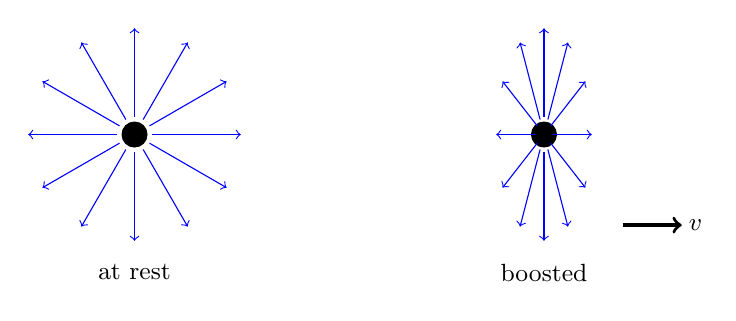
\begin{tikzpicture}[scale=1.0]
		\begin{scope}[shift={(-2.6,0)}]
			\node[draw, circle, inner sep=0.5pt, minimum size=9pt, fill=black] at (0,0) {};
			\foreach \a in {0,30,...,330}
				\draw[blue, ->] (\a:0.22) -- (\a:1.35);
			\node[anchor=north, inner sep=4pt] at (0,-1.5) {\small at rest};
		\end{scope}
		\begin{scope}[shift={(2.6,0)}]
			\node[draw, circle, inner sep=0.5pt, minimum size=9pt, fill=black] at (0,0) {};
			\foreach \a in {0,30,...,330} {
				\draw[blue, ->] ({0.22*cos(\a)*0.45},{0.22*sin(\a)}) -- ({1.35*cos(\a)*0.45},{1.35*sin(\a)});
			}
			\draw[->, very thick] (1.0,-1.15) -- (1.75,-1.15) node[anchor=west, inner sep=2pt] {\small $\vv{v}$};
			\node[anchor=north, inner sep=4pt] at (0,-1.5) {\small boosted};
		\end{scope}
	\end{tikzpicture}
	\end{center}

	There is also a magnetic field, which one obtains from the same transformation rules:
	$$
	\vv{B}' = \frac{\mu_0 \gamma Q v}{4\pi \left(\gamma^2(x'+vt')^2+y'^2+z'^2\right)^{3/2}}\begin{pmatrix}0\\ z'\\ -y'\end{pmatrix},
	$$
	circulating around the direction of motion, as one would expect of a moving charge.

	As a historical aside: this squashing of the field of a moving charge was found by Lorentz by solving Maxwell's equations directly, before relativity existed, and it is precisely what led him to write down the transformations that bear his name.
\end{example}

\subsection{Lorentz Invariants}

Since $\vv{E}$ and $\vv{B}$ mix under boosts, it is natural to ask whether any combination of them is agreed upon by all observers. With index notation this is easy to answer: we need to contract all indices away.

The first candidate is the obvious one.

\begin{proposition}
	The quantity
	$$
	\frac{1}{2}F_{\mu\nu}F^{\mu\nu} = |\vv{B}|^2 - \frac{|\vv{E}|^2}{c^2}
	$$
	is Lorentz invariant.
\end{proposition}
\begin{proof}
	Invariance is automatic, since all indices are contracted. The evaluation is a direct computation from the matrices above: the electric entries appear as (something)$\times$($-$something), contributing negatively, and the magnetic ones contribute positively.
\end{proof}

For the second invariant we need a new object. Define the totally antisymmetric symbol in four dimensions,
$$
\varepsilon^{\mu\nu\rho\sigma} = \begin{cases} +1 & \mu\nu\rho\sigma \text{ an even permutation of } 0123,\\ -1 & \text{an odd permutation},\\ 0&\text{otherwise},\end{cases}
$$
the spacetime analogue of $\epsilon_{ijk}$. Is it a tensor? Transforming it gives another totally antisymmetric object, and (exactly as in $\R^3$) the space of such objects is one-dimensional, so $\varepsilon'^{\mu\nu\rho\sigma} = a\,\varepsilon^{\mu\nu\rho\sigma}$ for some constant $a$. Testing on a single component,
$$
\varepsilon'^{0123} = \Lambda^0{}_\kappa \Lambda^1{}_\lambda\Lambda^2{}_\alpha\Lambda^3{}_\beta \varepsilon^{\kappa\lambda\alpha\beta} = \det \Lambda,
$$
by the definition of the determinant. Lorentz transformations have $\det\Lambda = \pm 1$, and restricting to the ones continuously connected to the identity (rotations and boosts, but not reflections or time reversal) we have $\det\Lambda = 1$ and $\varepsilon$ is indeed invariant.

\begin{definition}[Dual field tensor]
	The \vocab{dual electromagnetic tensor} is
	$$
	\tilde F^{\mu\nu} = \frac{1}{2}\varepsilon^{\mu\nu\rho\sigma}F_{\rho\sigma} = \begin{pmatrix} 0 & -B_x & -B_y & -B_z\\ B_x & 0 & E_z/c & -E_y/c\\ B_y & -E_z/c & 0 & E_x/c\\ B_z & E_y/c & -E_x/c & 0\end{pmatrix}.
	$$
\end{definition}

The factor of $\tfrac12$ is there because each pair $\{\rho,\sigma\}$ is counted twice in the sum. Comparing with $F^{\mu\nu}$, the dual is obtained by the substitution
$$
\vv{E} \mapsto c\vv{B}, \qquad \vv{B}\mapsto -\vv{E}/c,
$$
and the reader should note the minus sign: the duality is like a rotation by ninety degrees, and doing it twice gives minus the identity. In particular $\tilde F_{\mu\nu}\tilde F^{\mu\nu} = -F_{\mu\nu}F^{\mu\nu}$, so contracting the dual with itself gives nothing new. Contracting it with $F$, however, does.

\begin{proposition}
	The quantity
	$$
	\frac{1}{4}\tilde F^{\mu\nu}F_{\mu\nu} = \frac{\vv{E}\cdot\vv{B}}{c}
	$$
	is Lorentz invariant.
\end{proposition}

So all observers agree on $|\vv{B}|^2 - |\vv{E}|^2/c^2$ and on $\vv{E}\cdot\vv{B}$. In particular, if the fields are perpendicular in one frame they are perpendicular in every frame, and if $|\vv{E}| = c|\vv{B}|$ in one frame -- as for a plane wave -- then the same holds in all frames.

\subsection{Maxwell's Equations in Covariant Form}

We now have everything we need to write down the theory in its final form.

\begin{theorem}[Maxwell's equations, relativistic form]
	Maxwell's four equations are equivalent to the pair
	$$
	\partial_\mu F^{\mu\nu} = \mu_0 J^\nu, \qquad \partial_\mu \tilde F^{\mu\nu} = 0.
	$$
\end{theorem}
\begin{proof}
	We check each equation component by component. Take the first, with $\nu = 0$. Since $F^{00} = 0$, only spatial $\mu$ contribute, and $F^{i0} = E_i/c$, so
	$$
	\partial_i F^{i0} = \nabla\cdot\left(\frac{\vv{E}}{c}\right) = \mu_0 J^0 = \mu_0 \rho c,
	$$
	i.e. $\nabla\cdot\vv{E} = \mu_0 c^2 \rho = \rho/\epsilon_0$, which is (M1). Taking instead $\nu = i$ spatial, the $\mu = 0$ term gives $\frac{1}{c}\partial_t(-E_i/c)$ and the spatial terms assemble into $(\nabla\times\vv{B})_i$, so
	$$
	-\frac{1}{c^2}\frac{\partial \vv{E}}{\partial t} + \nabla\times\vv{B} = \mu_0\vv{J},
	$$
	which is (M4).

	Now the second equation. With $\nu = 0$ we get $\partial_i \tilde F^{i0} = \nabla\cdot\vv{B} = 0$, which is (M2); with $\nu = i$ we get $\frac{\partial \vv{B}}{\partial t} + \nabla\times\vv{E} = \vv{0}$, which is (M3).
\end{proof}

Two equations, each one line long, replacing four. It is hard to overstate how much cleaner this is: the constants $c$, $\epsilon_0$, $\mu_0$ have been almost entirely absorbed into the definitions, and the equations are manifestly Lorentz covariant, since both sides carry a single free upper index and so transform the same way.

Several facts we worked for now become immediate.

First, charge conservation. Since $F^{\mu\nu}$ is antisymmetric and $\partial_\nu\partial_\mu$ is symmetric, $\partial_\nu\partial_\mu F^{\mu\nu} = 0$ identically, and hence
$$
\partial_\nu J^\nu = 0.
$$
Compare this with the fiddly computation we did in Section~\ref{sec:displacement}.

Secondly, the second equation is automatic once we have potentials. If $F_{\mu\nu} = \partial_\mu A_\nu - \partial_\nu A_\mu$ then
$$
\partial_\mu \tilde F^{\mu\nu} = \frac{1}{2}\varepsilon^{\mu\nu\rho\sigma}\partial_\mu F_{\rho\sigma} = \frac{1}{2}\varepsilon^{\mu\nu\rho\sigma}\partial_\mu(\partial_\rho A_\sigma - \partial_\sigma A_\rho) = 0,
$$
since $\varepsilon$ is antisymmetric in $\mu\rho$ while $\partial_\mu\partial_\rho$ is symmetric. So the entire theory reduces to
$$
\partial_\mu F^{\mu\nu} = \mu_0 J^\nu \quad \text{where}\quad F_{\mu\nu} = \partial_\mu A_\nu - \partial_\nu A_\mu.
$$

Thirdly, the asymmetry between the two equations -- a source on one, zero on the other -- is exactly the statement that there are electric charges but no magnetic ones.

\subsection{The Lorenz Gauge}

In magnetostatics we exploited the freedom in $\vv{A}$ by choosing Coulomb gauge, $\nabla\cdot\vv{A} = 0$, which turned the field equation into Poisson's equation. There is a relativistic version of the same trick, and it is prettier.

\begin{definition}[Lorenz gauge]
	A gauge potential satisfying
	$$
	\partial_\mu A^\mu = 0
	$$
	is said to be in \vocab{Lorenz gauge}\footnote{After Ludvig Lorenz, who is not Hendrik Lorentz of the Lorentz transformations. The near-coincidence of names is one of the crueller accidents in the history of physics.}. In three-dimensional language this reads $\nabla\cdot\vv{A} + \frac{1}{c^2}\frac{\partial \phi}{\partial t} = 0$.
\end{definition}

Unlike Coulomb gauge, this condition is Lorentz invariant: it involves only a contracted pair of indices, so an observer in any frame will agree that it holds.

\begin{proposition}
	Any gauge potential can be brought into Lorenz gauge.
\end{proposition}
\begin{proof}
	Suppose $\partial_\mu A^\mu = \psi$. Under a gauge transformation $A_\mu \mapsto A_\mu - \partial_\mu \chi$ we get
	$$
	\partial_\mu A^\mu \mapsto \psi - \partial_\mu \partial^\mu \chi,
	$$
	so we need to solve $\Box \chi = \psi$, where $\Box = \partial_\mu\partial^\mu = \frac{1}{c^2}\frac{\partial^2}{\partial t^2} - \nabla^2$ is the \vocab{d'Alembertian}. This is the inhomogeneous wave equation, which always has solutions.
\end{proof}

The payoff is immediate. Substituting $F^{\mu\nu} = \partial^\mu A^\nu - \partial^\nu A^\mu$ into the Maxwell equation,
$$
\mu_0 J^\nu = \partial_\mu F^{\mu\nu} = \partial_\mu \partial^\mu A^\nu - \partial^\nu(\partial_\mu A^\mu) = \Box A^\nu,
$$
the second term vanishing precisely because we are in Lorenz gauge. So the whole of electromagnetism reduces to

\begin{theorem}
	In Lorenz gauge, Maxwell's equations are
	$$
	\Box A^\nu = \mu_0 J^\nu.
	$$
\end{theorem}

Four decoupled wave equations, one for each component of the potential, sourced by the corresponding component of the current. In empty space $J^\nu = \vv{0}$ and this is $\Box A^\nu = 0$: the potential propagates as a wave at speed $c$, which is our electromagnetic waves reappearing in a much more economical form. And the fact that the equation is a \emph{wave} equation rather than Poisson's equation says something physically important -- changing a charge here does not instantaneously change the field there. Influence propagates at the speed of light.

\begin{remark}
	The Lorenz gauge does not fix $A^\mu$ completely. We may still perform a further gauge transformation with any $\chi$ satisfying $\Box \chi = 0$, and remain in Lorenz gauge. This residual freedom is what allows one to argue that an electromagnetic wave has only two physical polarisation states, rather than the four one might naively count from $A^\mu$ -- exactly the two we found in Section~4.
\end{remark}

\subsection{The Lorentz Force in Covariant Form}

One thing remains: the force law. In non-relativistic notation it is
$$
\frac{\dd \vv{p}}{\dd t} = q(\vv{E}+\vv{u}\times\vv{B}),
$$
and we should like a version which is manifestly covariant. The right hand side involves $\vv{E}$, $\vv{B}$ and $\vv{u}$, which we now know how to package as $F^{\mu\nu}$ and $U^\mu$; the left is a rate of change of momentum, which becomes $\dd P^\mu/\dd\tau$. There is essentially only one way to combine these.

\begin{law}[Lorentz force law, relativistic form]
	A particle of charge $q$ obeys
	$$
	\frac{\dd P^\mu}{\dd \tau} = q\, F^{\mu\nu}U_\nu.
	$$
\end{law}

\begin{proposition}
	This is equivalent to the Lorentz force law together with the work-energy relation.
\end{proposition}
\begin{proof}
	Take $\mu = i$ spatial. Using $U_\nu = \gamma(c, -\vv{u})$ and reading off $F^{i\nu}$ from the matrix,
	$$
	\frac{\dd \vv{p}}{\dd \tau} = q\gamma(\vv{E} + \vv{u}\times\vv{B}),
	$$
	and since $\dd t/\dd\tau = \gamma$, the chain rule gives
	$$
	\frac{\dd \vv{p}}{\dd t} = q(\vv{E}+\vv{u}\times\vv{B}),
	$$
	the familiar law -- with the understanding that $\vv{p} = m\gamma\vv{u}$ is the relativistic momentum.

	Now take $\mu = 0$. Then $F^{0\nu}U_\nu = -\frac{\vv{E}}{c}\cdot(-\gamma\vv{u}) = \frac{\gamma}{c}\vv{E}\cdot\vv{u}$, so
	$$
	\frac{\dd P^0}{\dd\tau} = \frac{1}{c}\frac{\dd E}{\dd \tau} = \frac{q\gamma}{c}\vv{E}\cdot\vv{u} \implies \frac{\dd E}{\dd t} = q\vv{E}\cdot\vv{u},
	$$
	which is the statement that the electric field does work at a rate $q\vv{E}\cdot\vv{u}$ -- and, incidentally, that the magnetic field does none.
\end{proof}

So the time component of the covariant force law, which has no non-relativistic analogue as a separate statement, is the energy equation. This is a recurring theme in relativity: equations that look independent in three dimensions turn out to be components of a single four-dimensional statement.

We close with two standard applications.

\begin{example}[Motion in a constant electric field]
	Take $\vv{E} = (E,0,0)$ and start the particle from rest, so the motion stays along $\hh{x}$. The equation of motion is
	$$
	m\frac{\dd(\gamma u)}{\dd t} = qE \implies m\gamma u = qEt,
	$$
	taking $u = 0$ at $t=0$. Solving for $u$,
	$$
	u = \frac{\dd x}{\dd t} = \frac{qEt}{\sqrt{m^2 + q^2E^2t^2/c^2}}.
	$$
	Note that $u \to c$ as $t \to \infty$, but never reaches it: no amount of pushing gets a massive particle to the speed of light. Integrating,
	$$
	x = \frac{mc^2}{qE}\left(\sqrt{1 + \frac{q^2E^2t^2}{m^2c^2}} - 1\right),
	$$
	and for small $t$ this expands as $x \approx \frac{qE}{2m}t^2$, which is the Newtonian answer, as it must be.
\end{example}

\begin{example}[Motion in a constant magnetic field]
	Take $\vv{B} = (0,0,B)$ with $\vv{E} = \vv{0}$. The $\mu = 0$ equation gives
	$$
	\frac{\dd P^0}{\dd\tau} = 0 \implies E = m\gamma c^2 \text{ is constant},
	$$
	so $\gamma$, and hence $|\vv{u}|$, is constant -- as we knew, since magnetic fields do no work. The spatial equation is then
	$$
	m\gamma \frac{\dd \vv{u}}{\dd t} = q\vv{u}\times\vv{B},
	$$
	the $\gamma$ coming outside the derivative because it is constant. This is the equation we solved in Dynamics and Relativity, except for the factor of $\gamma$: the particle moves in a circle (or a helix, if it also has velocity along $\vv{B}$) with angular frequency
	$$
	\omega = \frac{qB}{m\gamma}.
	$$
	The relativistic correction is what makes a cyclotron stop working at high energies, and is why one builds synchrotrons instead.
\end{example}

That is the end of the course. It is worth taking stock of where we have got to. We began with four experimental laws about wires and magnets and charges, wrote them as differential equations, and found that they contained -- as inevitable consequences -- the existence of light, the impossibility of magnetic monopoles, the conservation of charge, and finally the structure of spacetime itself. Very little in mathematics repays this kind of attention so generously.

